%%%%%%%%%%%%%%%%%%%%%%%%%%%%%%%%%%%%%%%%%%%%%%%%%%%%%%%%%%%%%%%%%%%%%%
% Overleaf (WriteLaTeX) Example: Molecular Chemistry Presentation
%
% Source: http://www.overleaf.com
%
% In these slides we show how Overleaf can be used with standard 
% chemistry packages to easily create professional presentations.
% 
% Feel free to distribute this example, but please keep the referral
% to overleaf.com
% 
%%%%%%%%%%%%%%%%%%%%%%%%%%%%%%%%%%%%%%%%%%%%%%%%%%%%%%%%%%%%%%%%%%%%%%

\documentclass{beamer}

\mode<presentation>
{
  \usetheme{Madrid}       % or try default, Darmstadt, Warsaw, ...
  \usecolortheme{default} % or try albatross, beaver, crane, ...
  \usefonttheme{default}    % or try default, structurebold, ...
  \setbeamertemplate{navigation symbols}{}
  \setbeamertemplate{caption}[numbered]
} 

\usepackage[english]{babel}
\usepackage[utf8x]{inputenc}
\usepackage{graphicx}
\usepackage{hyperref}
  \hypersetup{colorlinks=true}
  \hypersetup{urlcolor=blue}
  \hypersetup{linkcolor = .}
\usepackage{xcolor}
\usepackage{siunitx}
  \sisetup{separate-uncertainty = true}
\usepackage{physics}
\usepackage[font=small,labelfont=bf]{caption}
\usepackage{subcaption}
\usepackage[en-GB]{datetime2}
\usepackage{overpic}
\usepackage{feynmp}
\DeclareGraphicsRule{*}{mps}{*}{}
\usepackage{scalerel}
\newcommand{\mylbrace}[2]{\vspace{#2pt}\hspace{6pt}\scaleleftright[\dimexpr5pt+#1\dimexpr0.06pt]{\lbrace}{\rule[\dimexpr2pt-#1\dimexpr0.5pt]{-4pt}{#1pt}}{.}}
\newcommand{\myrbrace}[2]{\vspace{#2pt}\scaleleftright[\dimexpr5pt+#1\dimexpr0.06pt]{.}{\rule[\dimexpr2pt-#1\dimexpr0.5pt]{-4pt}{#1pt}}{\rbrace}\hspace{6pt}}

% Here's where the presentation starts, with the info for the title slide
\title[$B^\pm\to(K^+K^-\pi^+\pi^-)_Dh^\pm$]{Model-independent (sort of) determination of the CKM angle \texorpdfstring{$\gamma$}{gamma} in \texorpdfstring{$B^\pm\to(K^+K^-\pi^+\pi^-)_Dh^\pm$}{B to K+K-pi+pi-} decays}

\author{\textbf{Martin Tat} \hspace{0.54em} Guy Wilkinson \hspace{0.54em} Sneha Malde}
\institute{\normalsize University of Oxford \\ \vspace{0.3cm} \normalsize B2OC Meeting, WG sign off \vspace{-0.2cm}}
\date{10th March 2022}

\titlegraphic{
\includegraphics[height = 2cm]{lhcb.jpg}\hspace{2cm}~%
              
\includegraphics[height = 2cm]{OxfordLogo.pdf}}

\begin{document}

\begin{frame}
  \titlepage
\end{frame}

% These three lines create an automatically generated table of contents.
\begin{frame}{Outline}
  \tableofcontents
\end{frame}

\section{Summary of \texorpdfstring{$\gamma$}{gamma} analysis in \texorpdfstring{$B^\pm\to Dh^\pm$, $D\to h^+h^-\pi^+\pi^-$}{B2Dh, D2hhpipi}}
\begin{frame}{Summary of $\gamma$ analysis in $B^\pm\to Dh^\pm$, $D\to h^+h^-\pi^+\pi^-$}
  \begin{center}
    {\huge Summary of $\gamma$ analysis in\\~\\$B^\pm\to Dh^\pm$, $D\to h^+h^-\pi^+\pi^-$}
  \end{center}
\end{frame}

\begin{frame}{Summary of $\gamma$ analysis in $B^\pm\to Dh^\pm$, $D\to h^+h^-\pi^+\pi^-$}
  \vspace{0.5cm}
  \begin{itemize}
    \setlength\itemsep{1.2em}
    \item{First presented to B2OC WG on 4th November 2022}
    \begin{itemize}
      \item{Slides \href{https://indico.cern.ch/event/1085269/\#7-b-dkkpipih}{here}}
      \item{TWiki page with ANA note \href{https://twiki.cern.ch/twiki/bin/view/LHCbPhysics/GGSZB2DhD2hhpipiModelIndependent}{here}}
    \end{itemize}
    \item{GGSZ: Analysis in phase space bins of $D^0\to K^+K^-\pi^+\pi^-$}
    \begin{itemize}
      \item{This publication: $c_i$/$s_i$ from LHCb model \href{https://arxiv.org/abs/1811.08304}{JHEP 02 (2019) 126}}
      \item{Long term plan: Strong-phase analysis at BESIII currently ongoing where $c_i$/$s_i$ are measured directly $\implies$ Model independent analysis}
    \end{itemize}
    \item{Quasi-GLW: Phase space integrated analysis of $D^0\to h^+h^-\pi^+\pi^-$}
    \begin{itemize}
      \item{$F_+^{4\pi} = 0.769 \pm 0.023$ from CLEO-c data \href{https://arxiv.org/abs/1709.03467}{JHEP 01 (2018) 144}}
      \item{$F_+^{KK\pi\pi} = 0.736$ from LHCb model}
      \begin{itemize}
        \item{Preliminary BESIII analysis of $F_+$ shows good agreement with model}
      \end{itemize}
    \end{itemize}
  \end{itemize}
\end{frame}

\begin{frame}{The BPGGSZ method}
  \begin{block}{Event yield in bin $i$}
    \scriptsize
    $N^-_i = h_{B^-}\big(F_i + (x_-^2 + y_-^2)\bar{F_i} + 2\sqrt{F_i\bar{F_i}}(x_-c_i + y_-s_i)\big)$ \\
    $N^+_{-i} = h_{B^+}\big(F_i + (x_+^2 + y_+^2)\bar{F_i} + 2\sqrt{F_i\bar{F_i}}(x_+c_i + y_+s_i)\big)$
  \end{block}
  \begin{itemize}
    \item{CP observables:}
    \begin{itemize}
      \item{$x_\pm^{DK} = r_B^{DK}\cos(\delta_B^{DK}\pm\gamma)$, \quad $y_\pm^{DK} = r_B^{DK}\sin(\delta_B^{DK}\pm\gamma)$}
      \item{$x_\xi^{D\pi} = \Re(\xi^{D\pi})$, $y_\xi^{D\pi} = \Im(\xi^{D\pi})$ $\quad\quad\Big(\xi^{D\pi} = \frac{r_B^{D\pi}}{r_B^{DK}}e^{i(\delta_B^{D\pi} - \delta_B^{DK})}\Big)$}
    \end{itemize}
    \item{Fractional bin yield:}
    \begin{itemize}
      \item{$F_i = \frac{\int_i\dd{\Phi}|\mathcal{A}(D^0)|^2}{\sum_j\int_j\dd{\Phi}\abs{\mathcal{A}(D^0)}^2}$}
      \item{Floated in the fit, mostly constrained by $B^\pm\to D\pi^\pm$}
    \end{itemize}
  \end{itemize}
  \begin{itemize}
    \item{Amplitude averaged strong phases:}
    \begin{center}
      $c_i = \frac{\int_i\dd{\Phi}|\mathcal{A}(D^0)||\mathcal{A}(\bar{D^0})|\cos(\delta_D)}{\sqrt{\int_i\dd{\Phi}\abs{\mathcal{A}(D^0)}^2\int_i\dd{\Phi}\abs{\mathcal{A}(\bar{D^0})}^2}}$ \quad $s_i = \frac{\int_i\dd{\Phi}|\mathcal{A}(D^0)||\mathcal{A}(\bar{D^0})|\sin(\delta_D)}{\sqrt{\int_i\dd{\Phi}\abs{\mathcal{A}(D^0)}^2\int_i\dd{\Phi}\abs{\mathcal{A}(\bar{D^0})}^2}}$
    \end{center}
  \end{itemize}
\end{frame}

\begin{frame}{Binning scheme}
  \begin{figure}
    \centering
    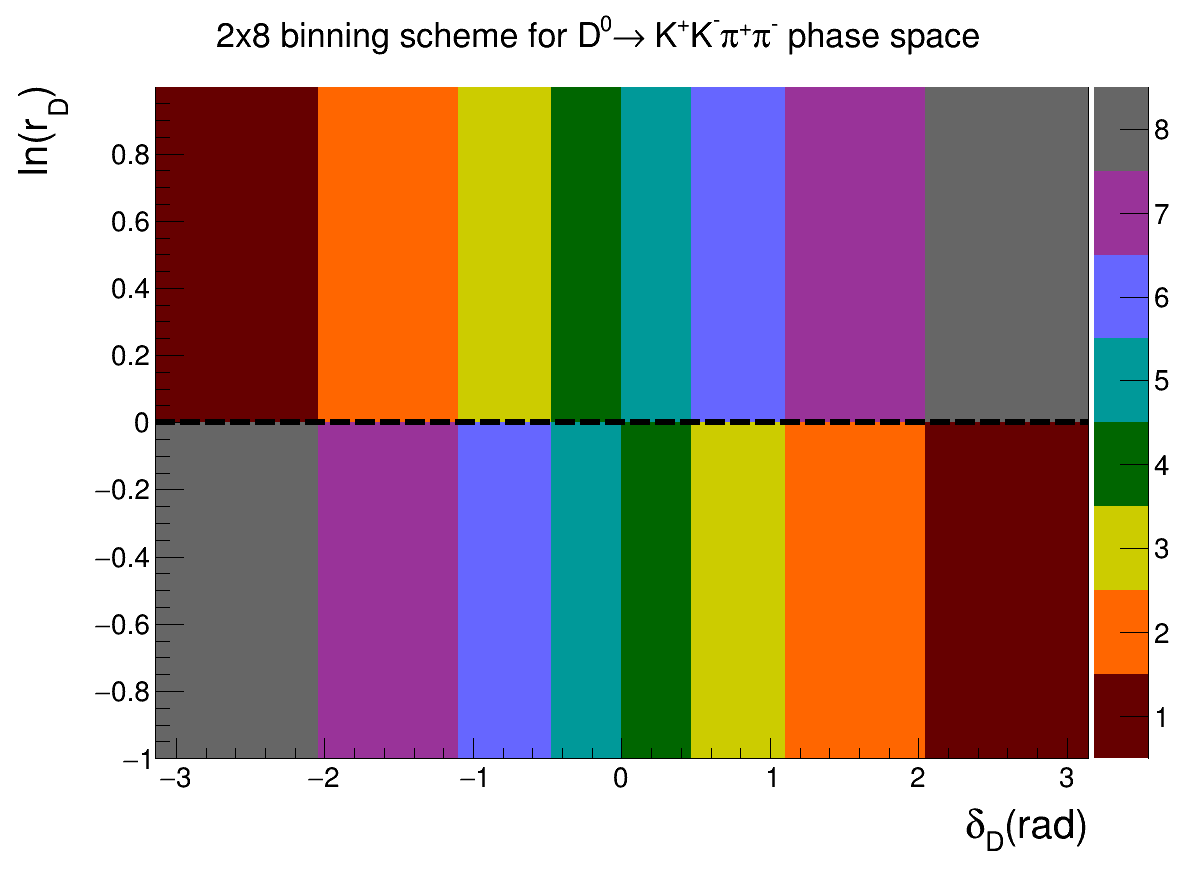
\includegraphics[width = 0.7\textwidth]{Plots/BinningSchemePlot_8Bins.png}
  \end{figure}
  \vspace{-1.0cm}
  \begin{center}
    $Q = 0.90$ \\
    Bins $i < 0$ on top, $i > 0$ below
  \end{center}
\end{frame}

\begin{frame}{The quasi-GLW method}
  \begin{itemize}
    \setlength\itemsep{0.5em}
    \item{Statistically independent analysis without phase space binning}
    \begin{itemize}
      \item{BPGGSZ looks at relative bin yields}
      \item{Quasi-GLW observables depend on absolute yields}
    \end{itemize}
    \item{Charge asymmetry:}
    \begin{center}
      $A_h = \frac{\Gamma(B^-\to D h^-) - \Gamma(B^+\to D h^+)}{\Gamma(B^-\to D h^-) + \Gamma(B^+\to D h^+)}$
    \end{center}
    \item{$B\to DK$ vs $B\to D\pi$ double ratio:}
    \begin{center}
      $R_{\rm CP} = \frac{R_{hh\pi\pi}}{R_{K\pi\pi\pi}}, \quad R = \frac{\Gamma(B^-\to D K^-) + \Gamma(B^+\to D K^+)}{\Gamma(B^-\to D\pi^-) + \Gamma(B^+\to D\pi^+)}$
    \end{center}
  \end{itemize}
  \begin{block}{CP observables and physics parameters}
    $A_h = \frac{2r_B^{Dh}(2F_+ - 1)\sin(\delta_B^{Dh})\sin(\gamma)}{1 + (r_B^{Dh})^2 + 2r_B^{Dh}(2F_+ - 1)\cos(\delta_B^{Dh})\cos(\gamma)}$, \\~\\
    $R_{\rm CP} = 1 + (r_B^{Dh})^2 + 2r_B^{Dh}(2F_+ - 1)\cos(\delta_B^{Dh})\cos(\gamma)$
  \end{block}
\end{frame}

\begin{frame}{Selection}
  \begin{enumerate}
    \setlength\itemsep{1.0em}
    \item{Initial cuts: Trigger requirements, mass cuts, bachelor $p$, etc}
    \item{BDT: Efficient combinatorial background rejection}
    \item{Final cuts: PID cuts, flight significance cuts, $K_S$ veto, etc}
  \end{enumerate}
  \vspace{0.5cm}
  \begin{figure}
    \centering
    \vspace{-0.2cm}
    \begin{subfigure}{0.5\textwidth}
      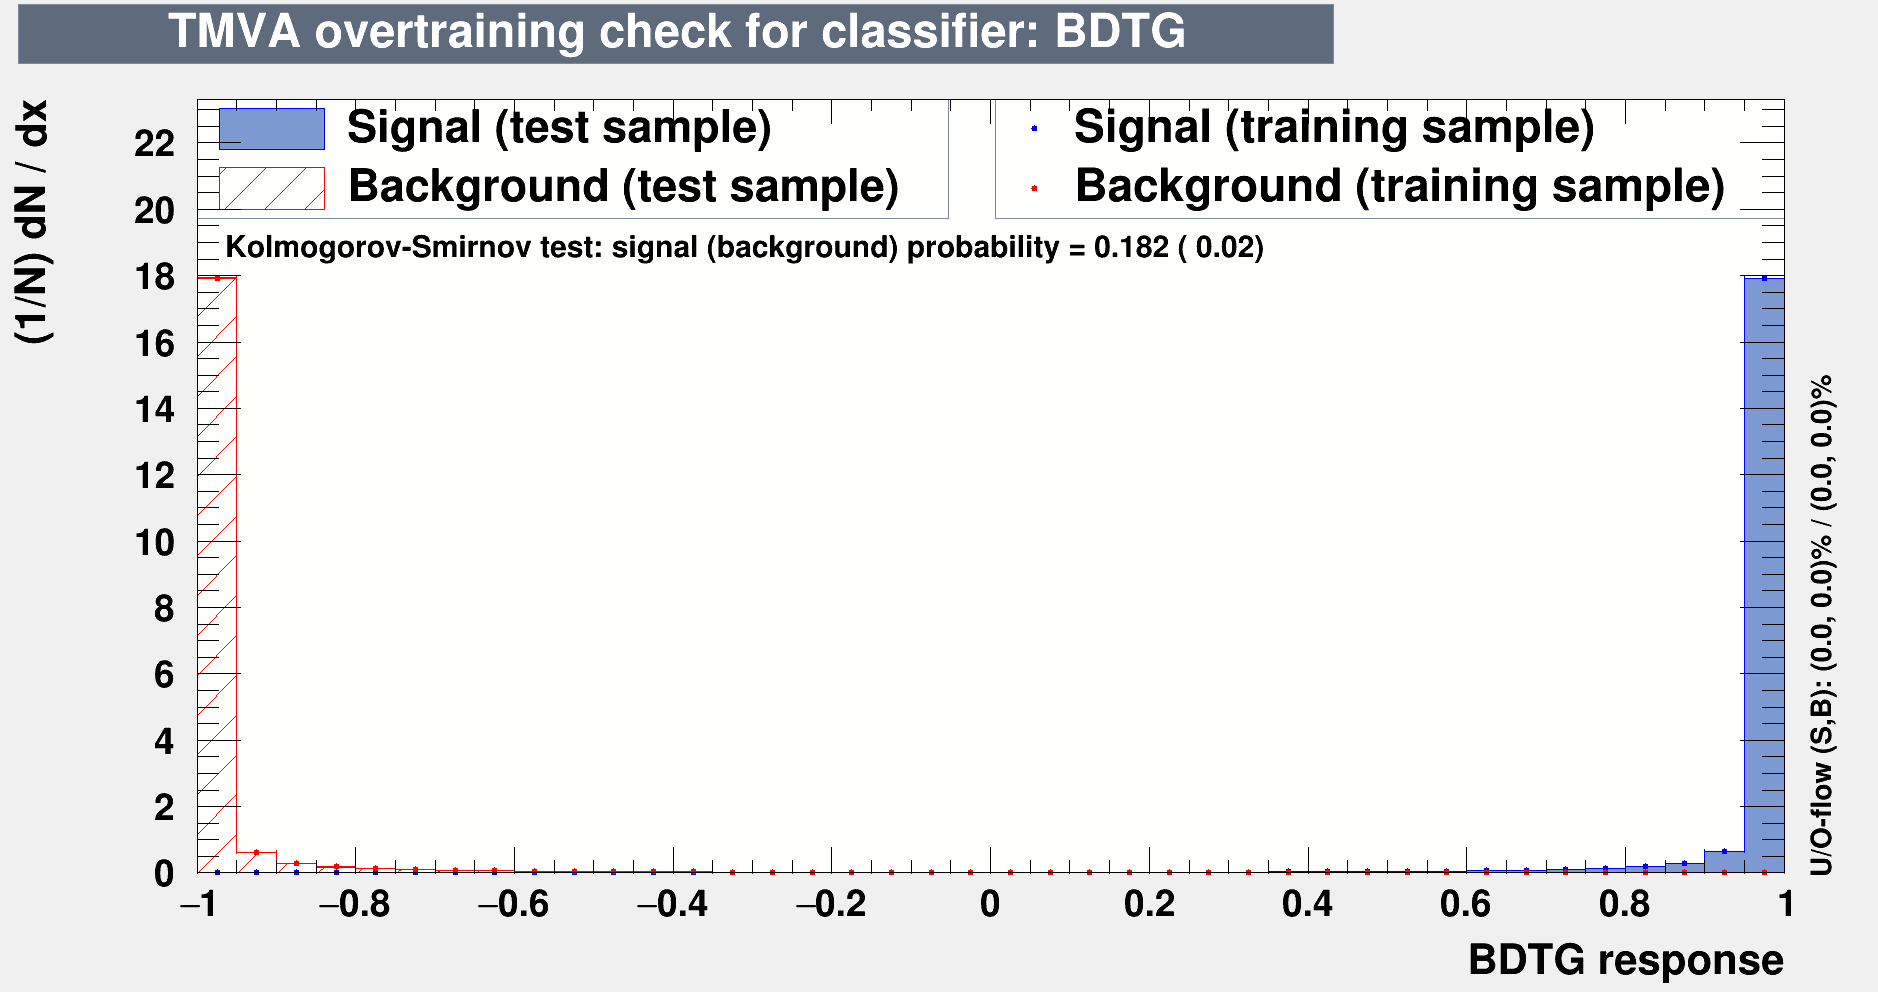
\includegraphics[width = 1.0\textwidth]{Plots/overtrain_BDTG.png}
      \caption{BDT output}
    \end{subfigure}%
    \begin{subfigure}{0.5\textwidth}
      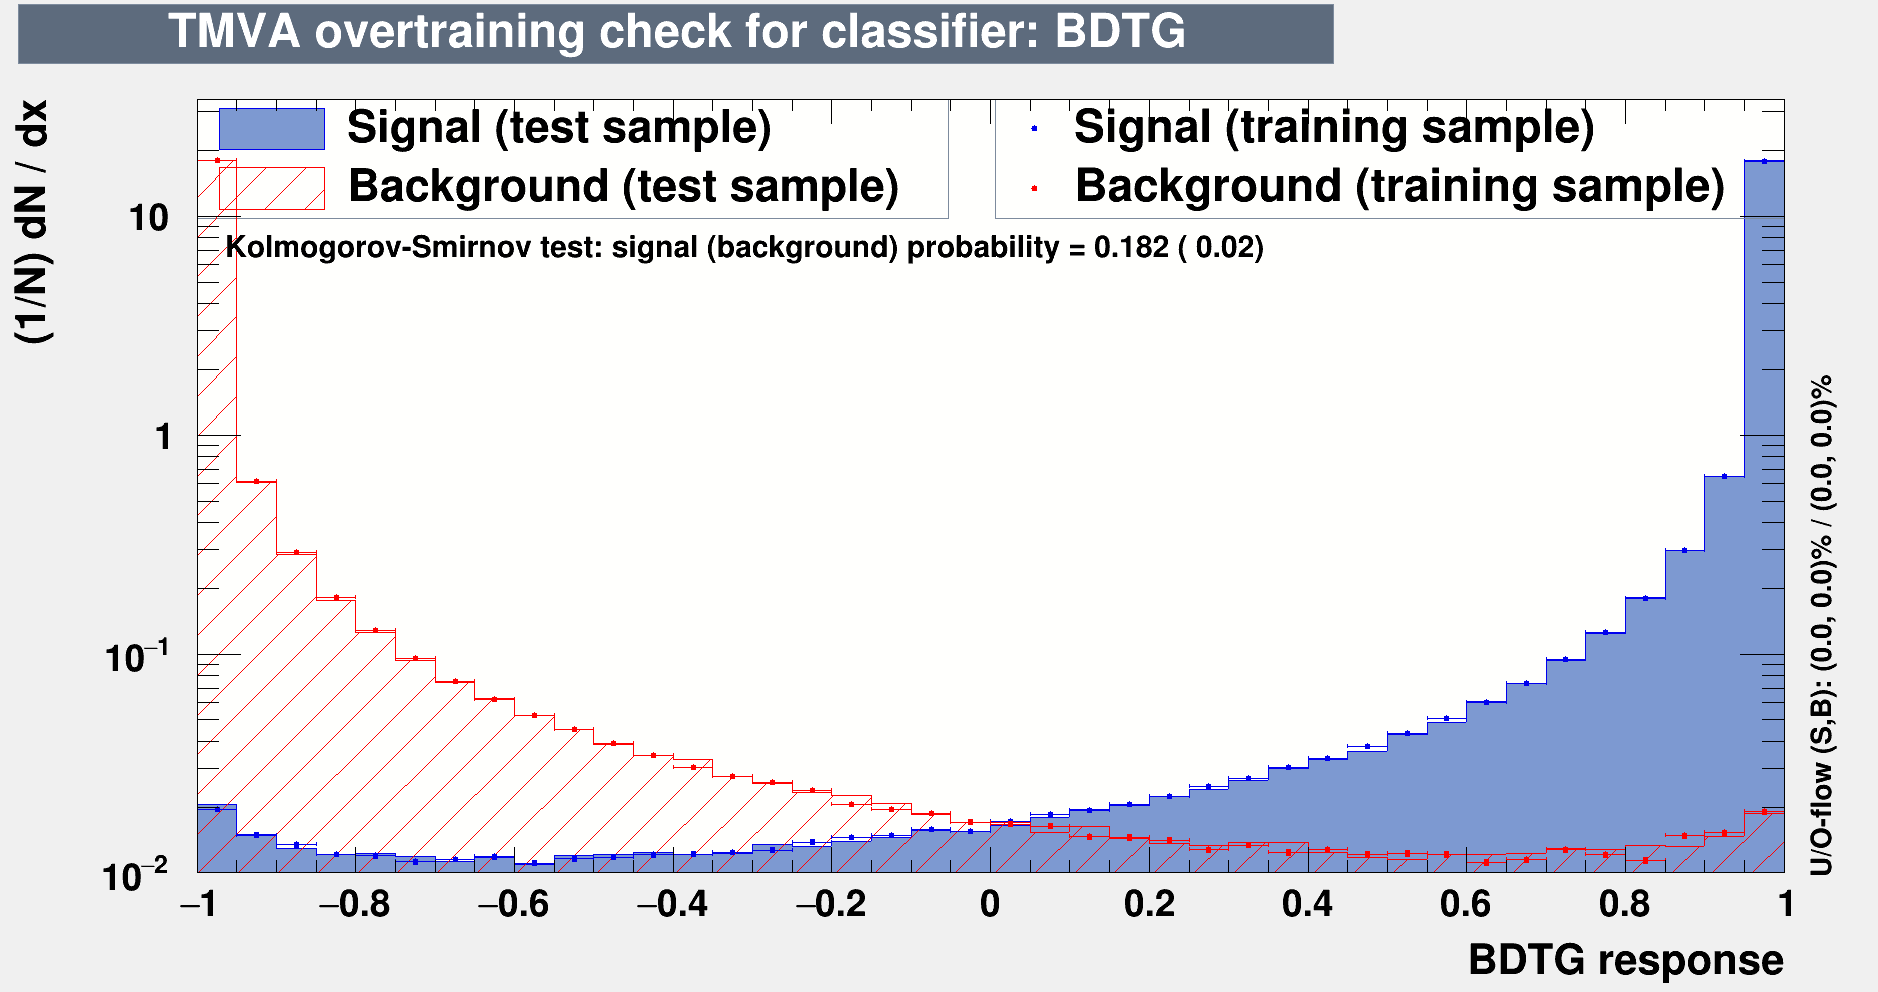
\includegraphics[width = 1.0\textwidth]{Plots/overtrain_BDTG_log.png}
      \caption{BDT output on a logarithmic scale}
    \end{subfigure}
  \end{figure}
\end{frame}

\begin{frame}{Global fit}
  \begin{figure}
    \centering
    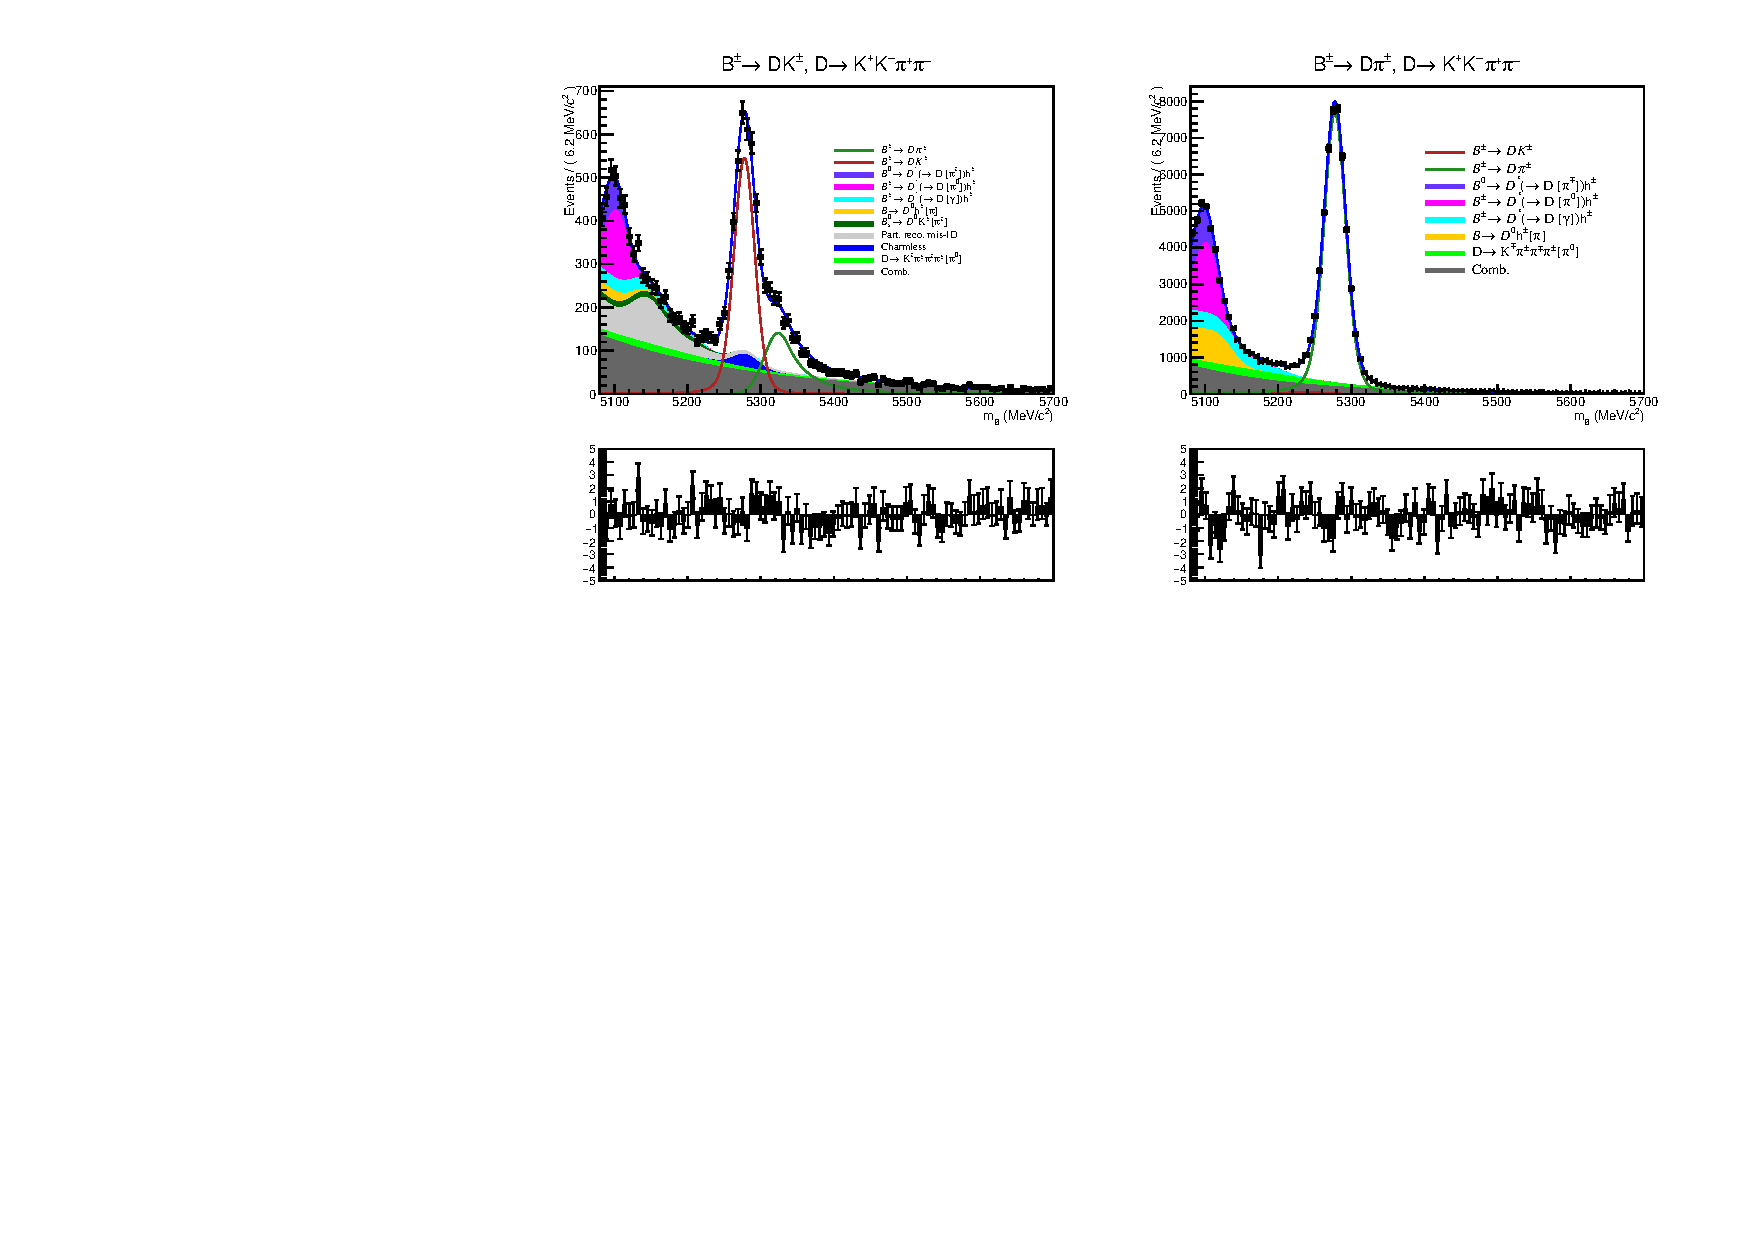
\includegraphics[width = 1.0\textwidth]{Plots/d2kkpipi_fiveL_allDP.pdf}
    \caption{$B^\pm\to DK^\pm$ channel (left) and $B^\pm\to D\pi^\pm$ channel (right)}
  \end{figure}
  \vspace{-0.5cm}
  \begin{itemize}
    \item{$B^\pm\to DK^\pm$ yield: $\SI{3306(75)}{}$}
    \item{$B^\pm\to D\pi^\pm$ yield: $\SI{46695(256)}{}$}
  \end{itemize}
\end{frame}

\begin{frame}{Fit split by charge}
  \begin{figure}
    \centering
    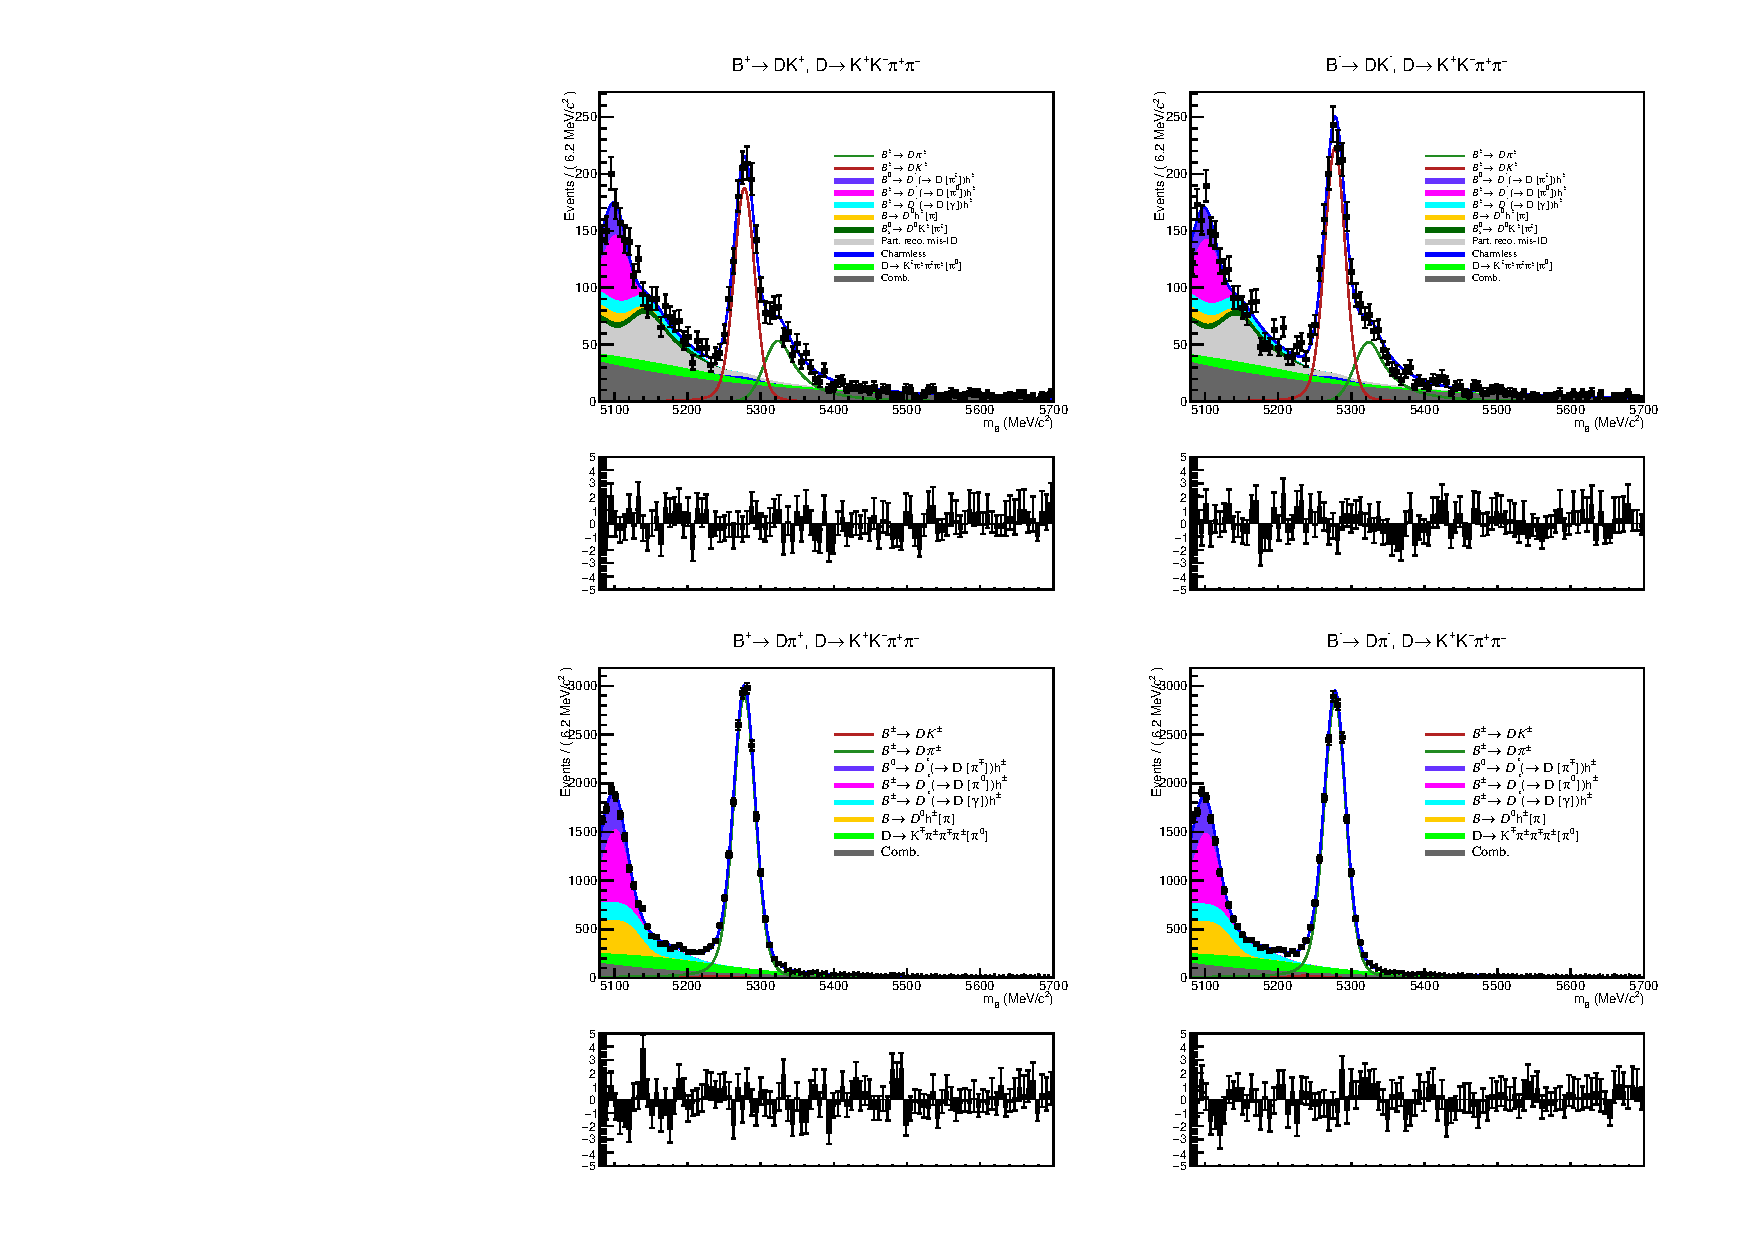
\includegraphics[width = 0.9\textwidth, clip = true, trim = {0 12.9cm 0 0}]{Plots/d2kkpipi_fiveL_allDP_GLW.pdf}
    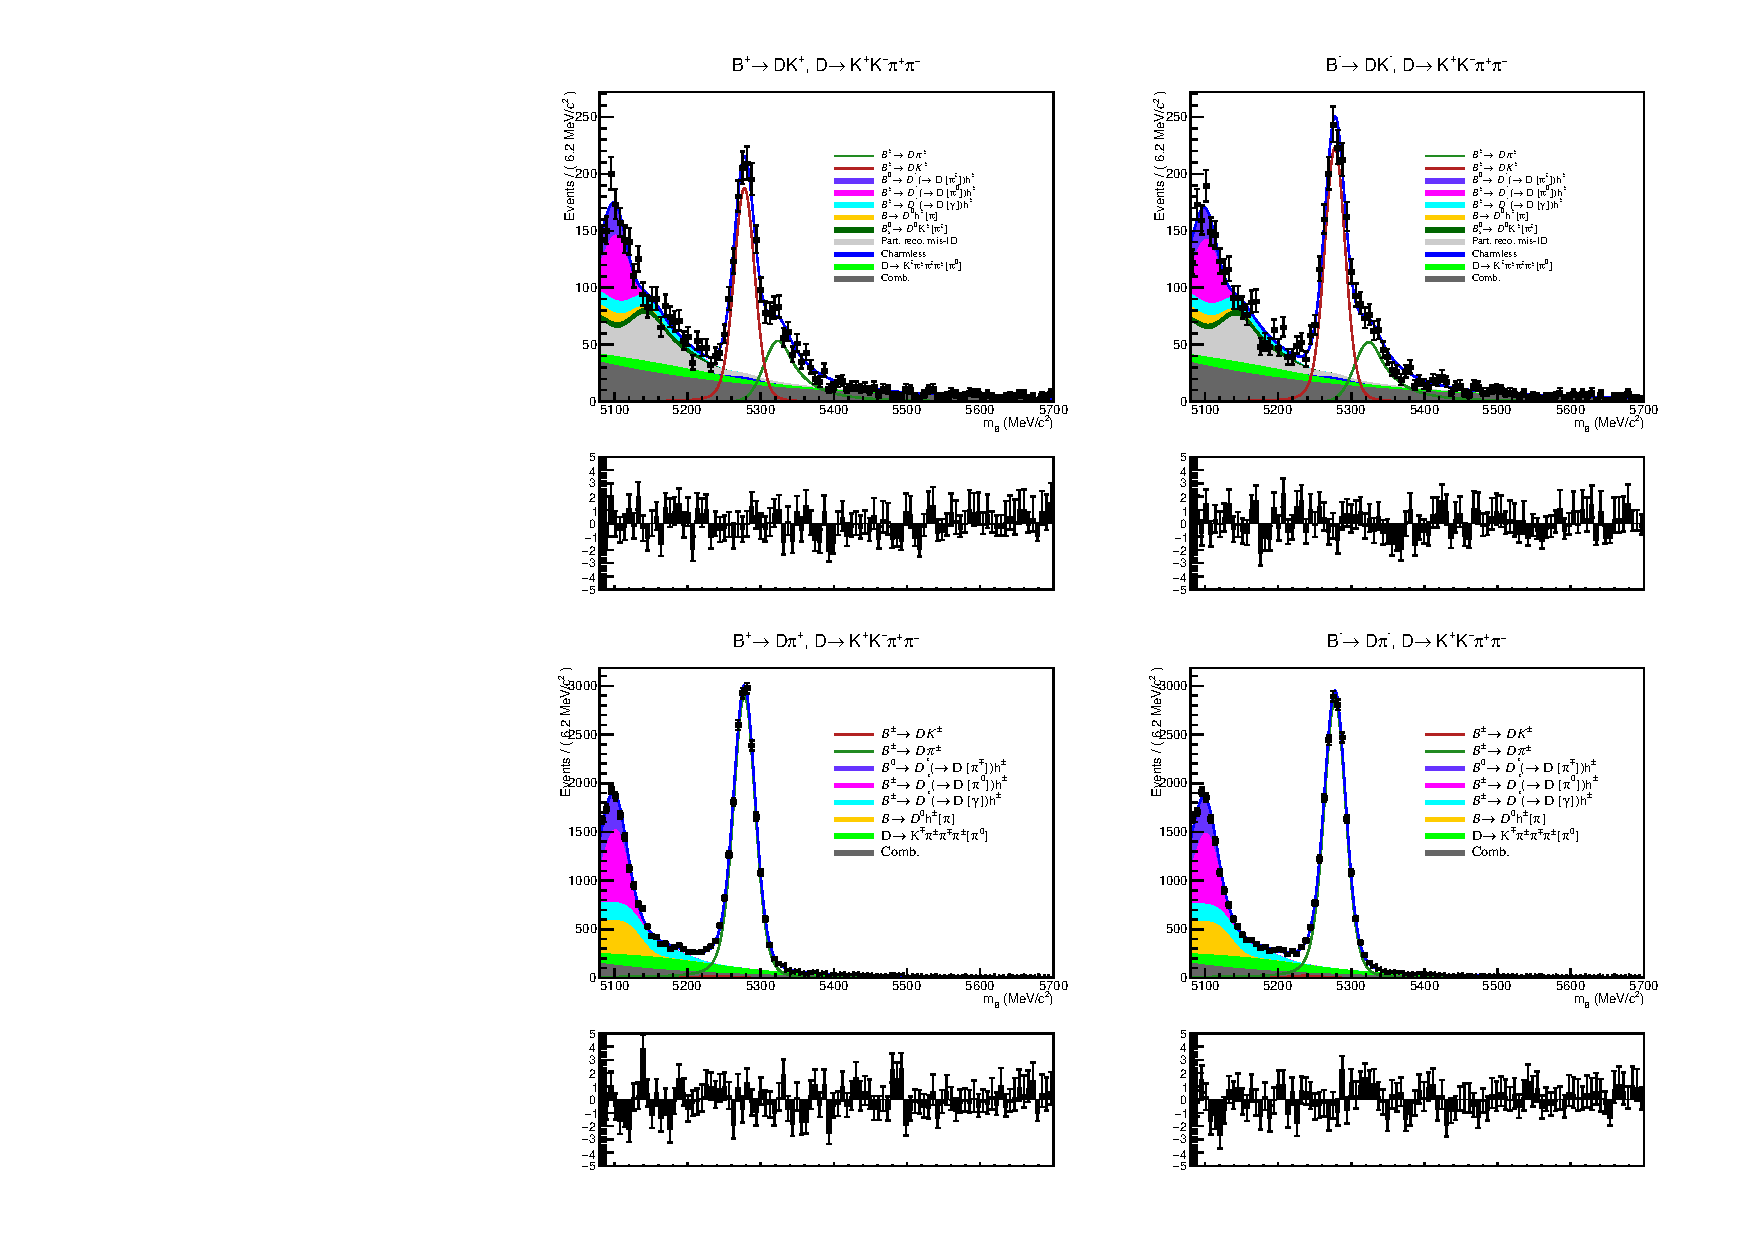
\includegraphics[width = 0.9\textwidth, clip = true, trim = {0 3cm 0 10cm}]{Plots/d2kkpipi_fiveL_allDP_GLW.pdf}
    \caption{$B^\pm\to (K^+K^-\pi^+\pi^-)Dh^\pm$}
  \end{figure}
\end{frame}

\begin{frame}{Fit split by charge}
  \begin{figure}
    \centering
    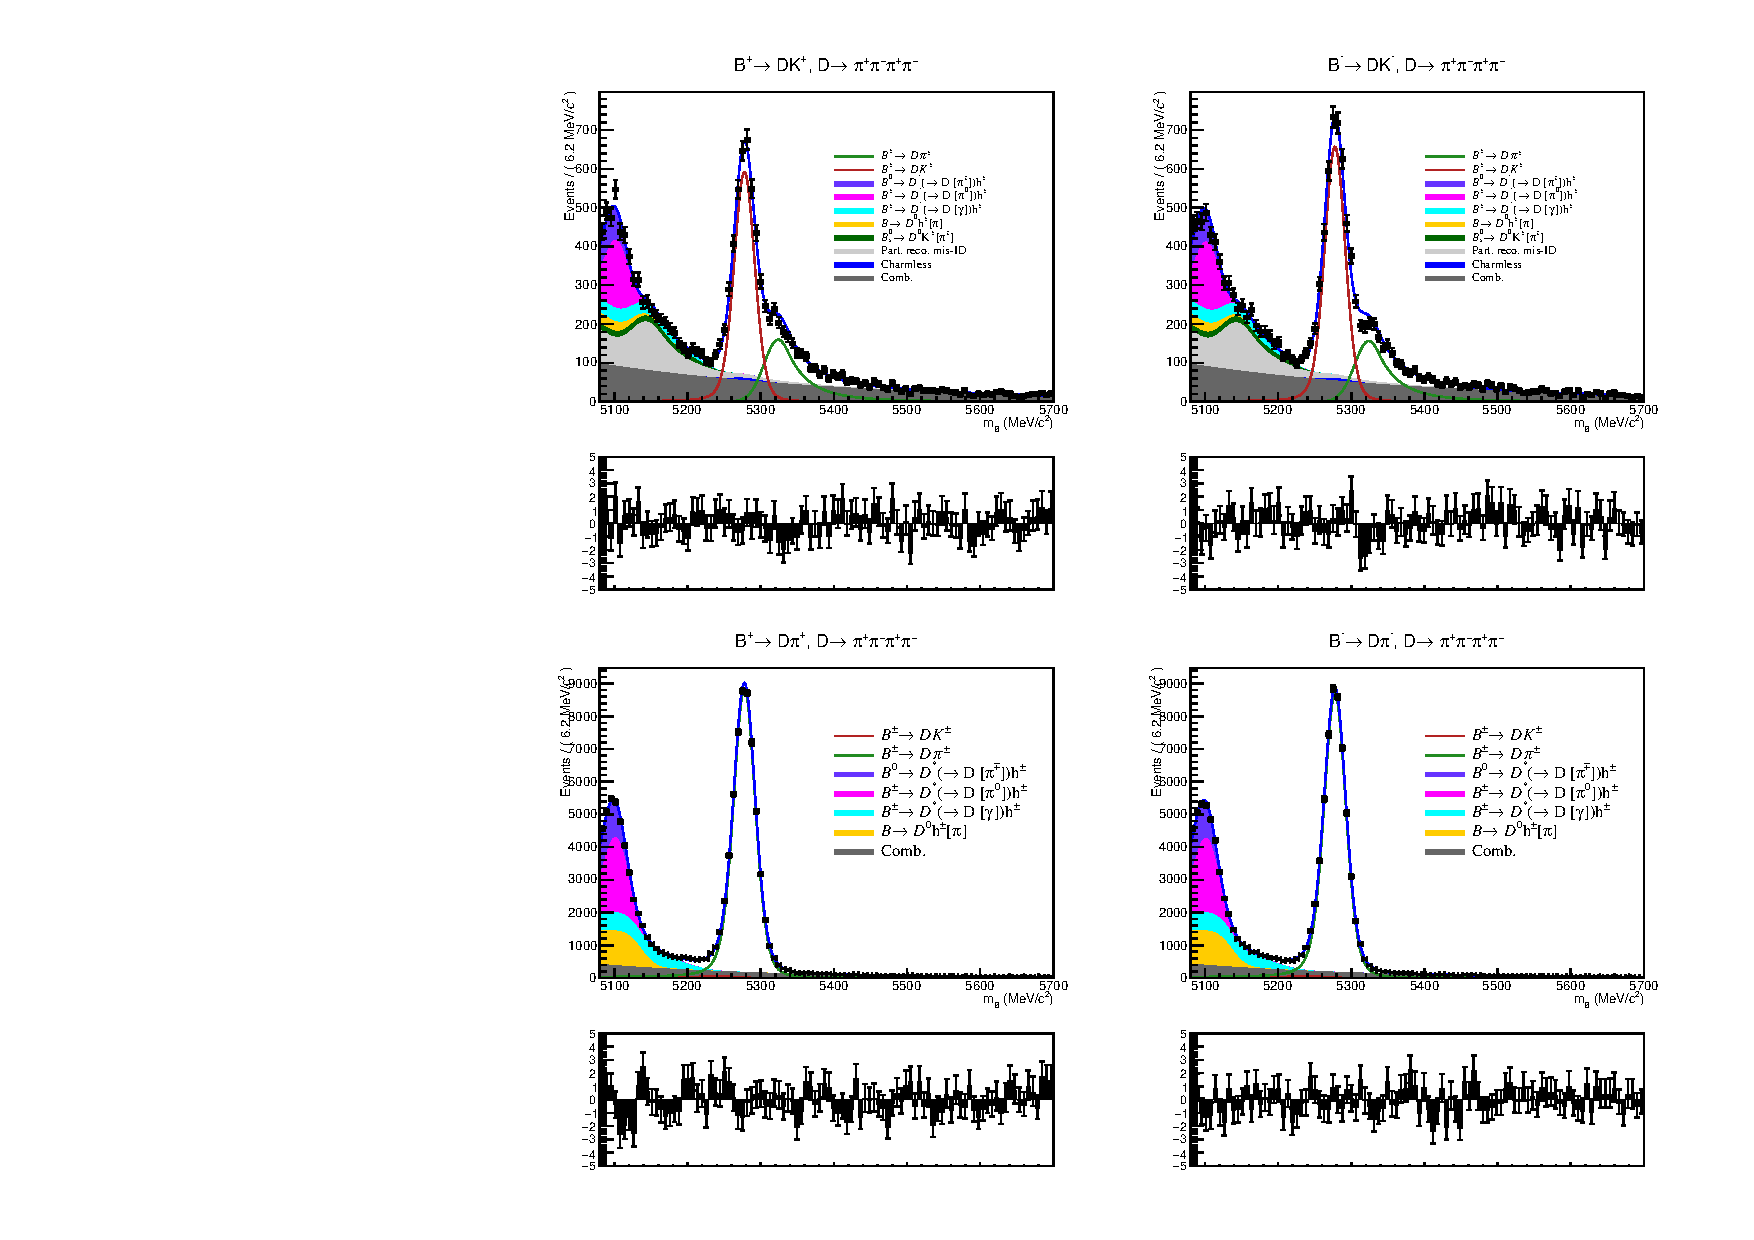
\includegraphics[width = 0.9\textwidth, clip = true, trim = {0 12.9cm 0 0}]{Plots/d2pipipipi_fiveL_allDP_GLW.pdf}
    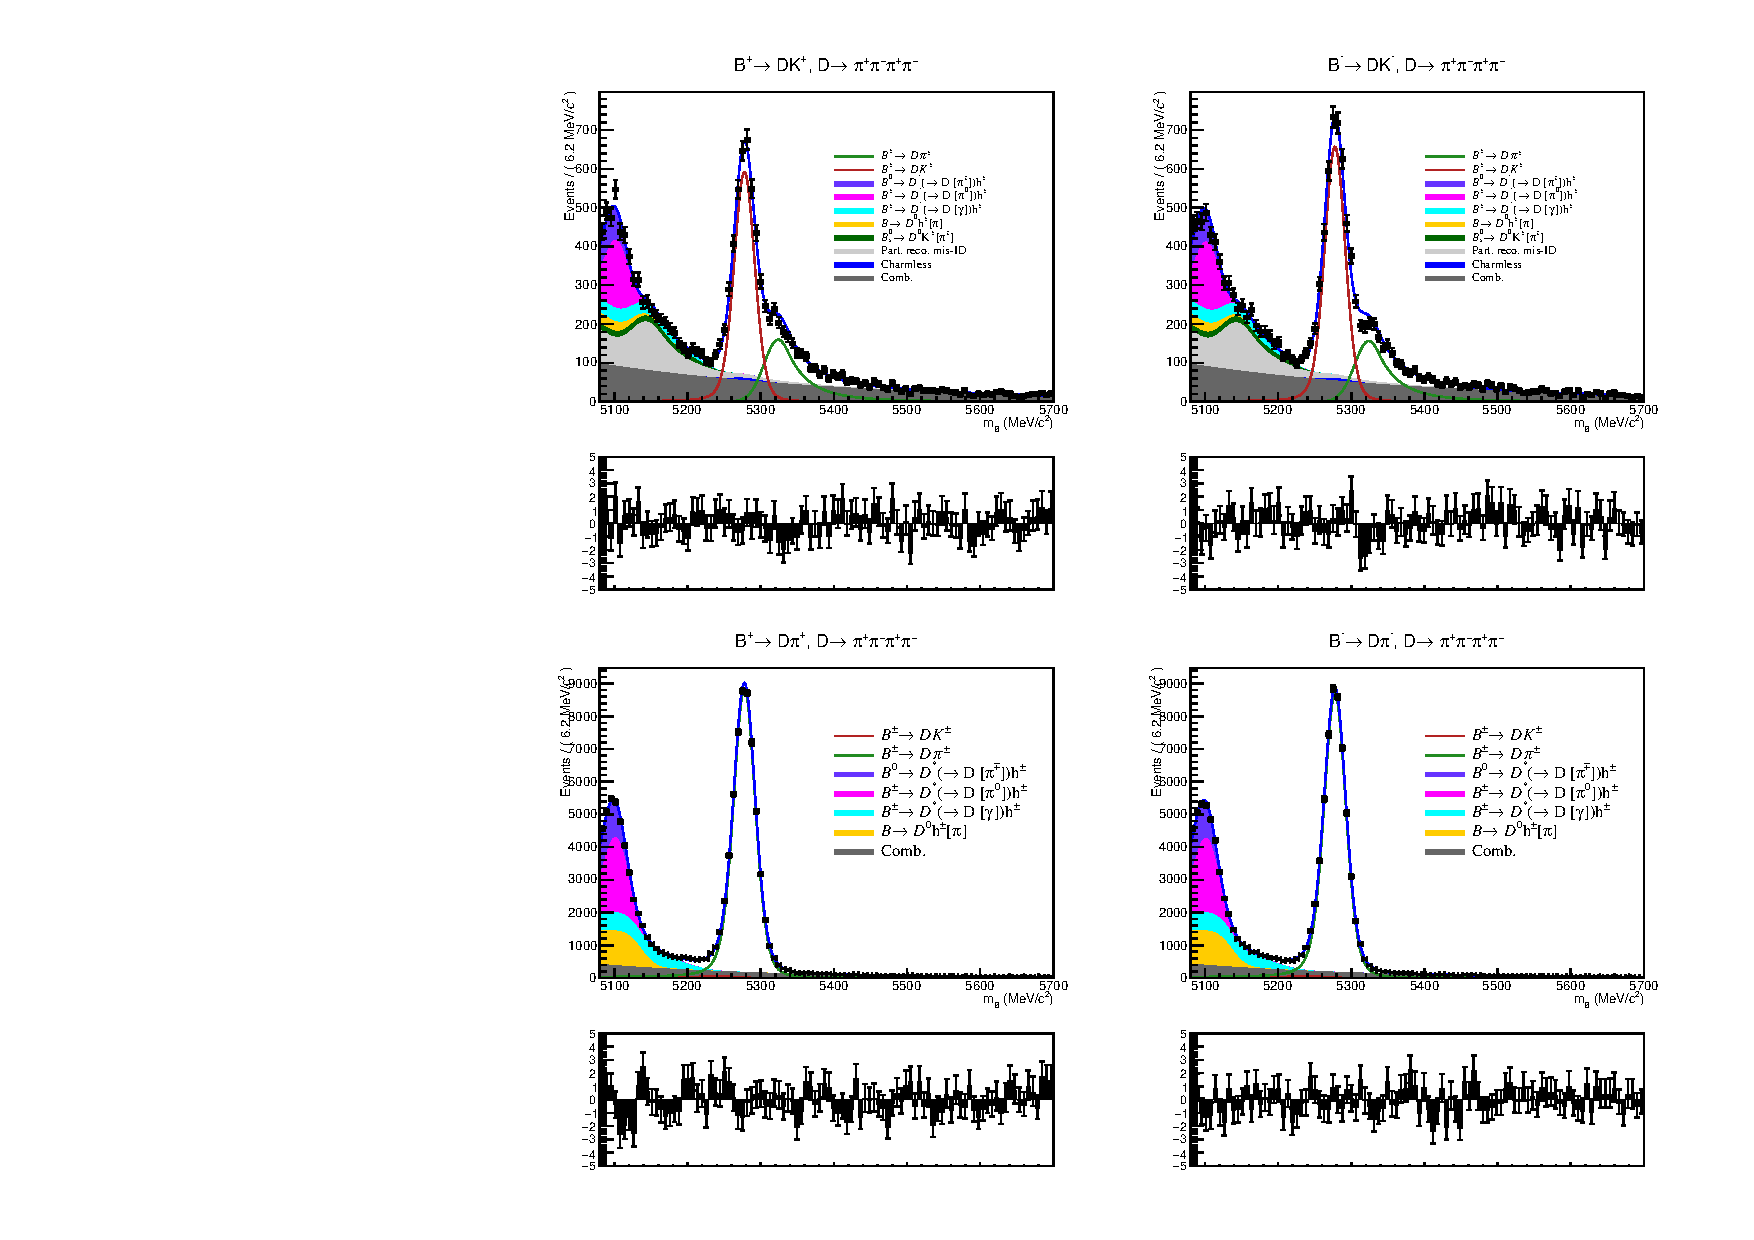
\includegraphics[width = 0.9\textwidth, clip = true, trim = {0 3cm 0 10cm}]{Plots/d2pipipipi_fiveL_allDP_GLW.pdf}
    \caption{$B^\pm\to (\pi^+\pi^-\pi^+\pi^-)Dh^\pm$}
  \end{figure}
\end{frame}

\section{Updates and improvements to analysis}
\begin{frame}{Updates and improvements to analysis}
  \begin{center}
    {\huge Updates and improvements to analysis}
  \end{center}
  \begin{center}
    \Large ~\\Thanks to Anton, Nathan, Paras\\for reading the ANA note!
  \end{center}
\end{frame}

\subsection{\texorpdfstring{$D\to K\pi\pi\pi\pi^0$}{D2Kpipipipi0} mis-ID background}
\begin{frame}{$D\to K\pi\pi\pi\pi^0$ mis-ID background}
  \begin{itemize}
    \setlength\itemsep{0.0em}
    \item{Missing $\pi^0$ and $\pi\to K$ mis-ID}
    \item{Two changes:}
    \begin{enumerate}
      \item{Unclear how DTF affects mass shape $\implies$ Requested LHCb MC}
      \item{Float yield relative to $B\to D^*h$ background instead of all partially reconstructed background}
    \end{enumerate}
    \item{Cross checks: Model dependence and bin dependence}
  \end{itemize}
  \begin{figure}
    \centering
    \begin{subfigure}{0.50\textwidth}
      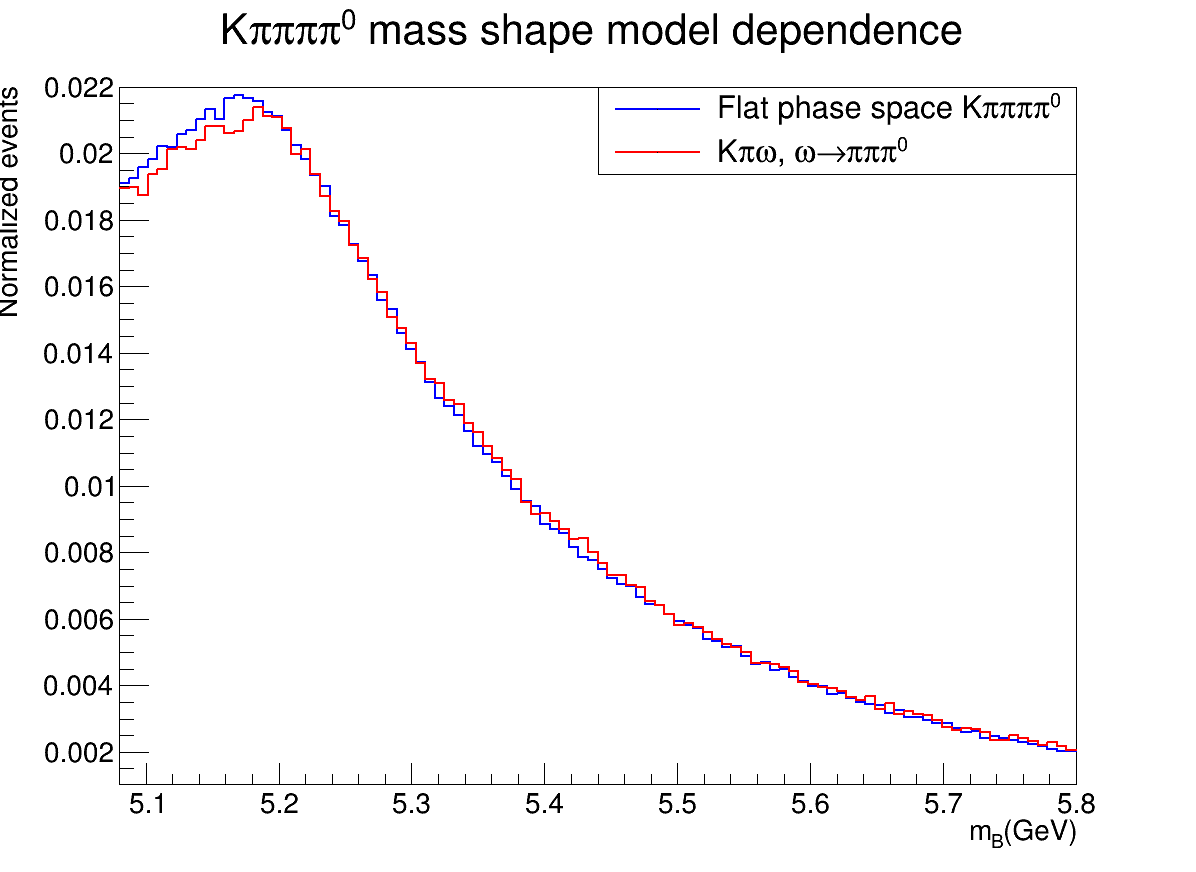
\includegraphics[width = 1.0\textwidth]{Plots/Kpipipipi0_mass_shape_model_dependence.png}
    \end{subfigure}%
    \begin{subfigure}{0.50\textwidth}
      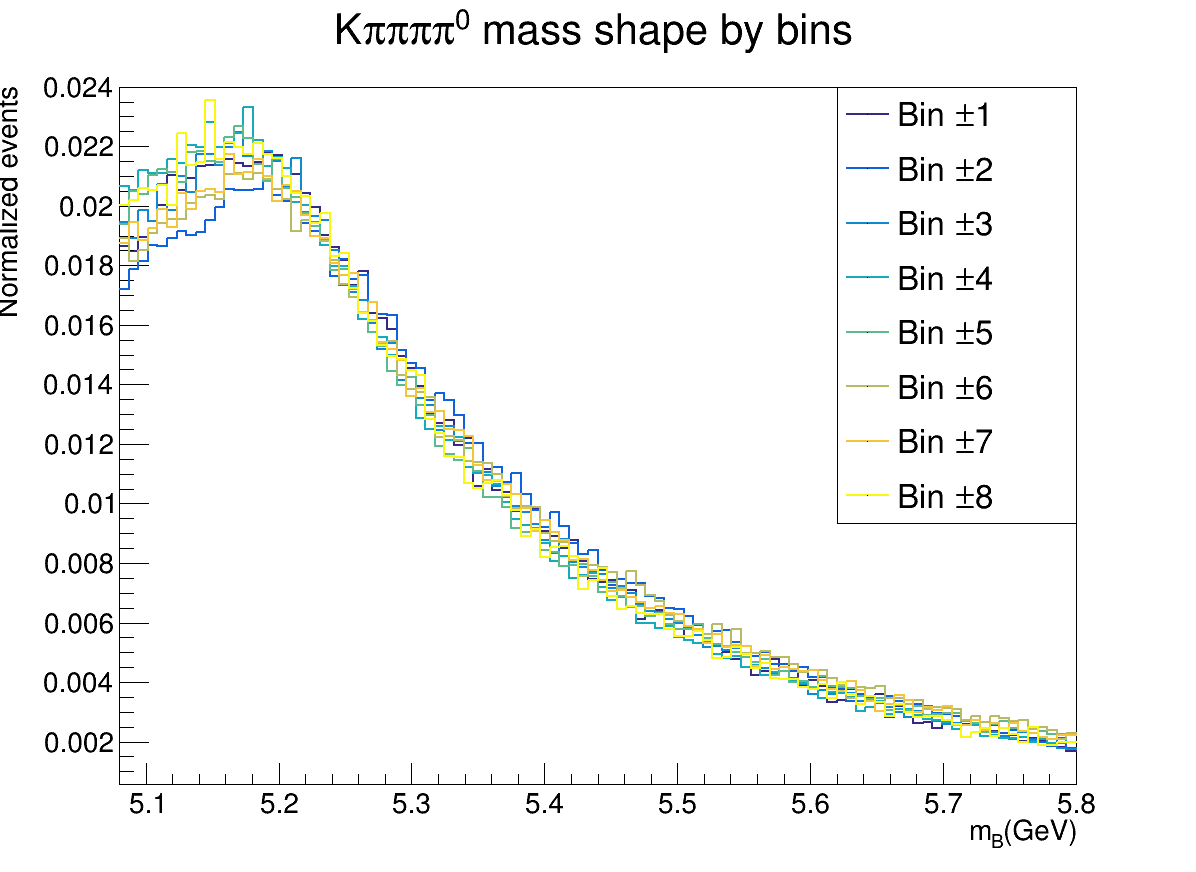
\includegraphics[width = 1.0\textwidth]{Plots/Kpipipipi0_mass_shape_by_bins.png}
    \end{subfigure}
  \end{figure}
\end{frame}

\begin{frame}{$D\to K\pi\pi\pi\pi^0$ mis-ID background}
  \begin{itemize}
    \setlength\itemsep{0.5em}
    \item{Reweighting procedure:}
    \begin{enumerate}
      \item{Run through same reconstruction as $KK\pi\pi$}
      \item{Use $KK\pi\pi$ MC to calculate PID efficiency of $\rm{PIDK} > -10$ as a function of $p$ and $\eta$}
      \item{Reweight each event to ``undo'' the PID cut from stripping}
      \item{Reweight with PIDCalib2 to account for $\rm{PIDK} > 0$ cut in selection}
    \end{enumerate}
  \end{itemize}
  \begin{figure}
    \centering
    \begin{subfigure}{0.50\textwidth}
      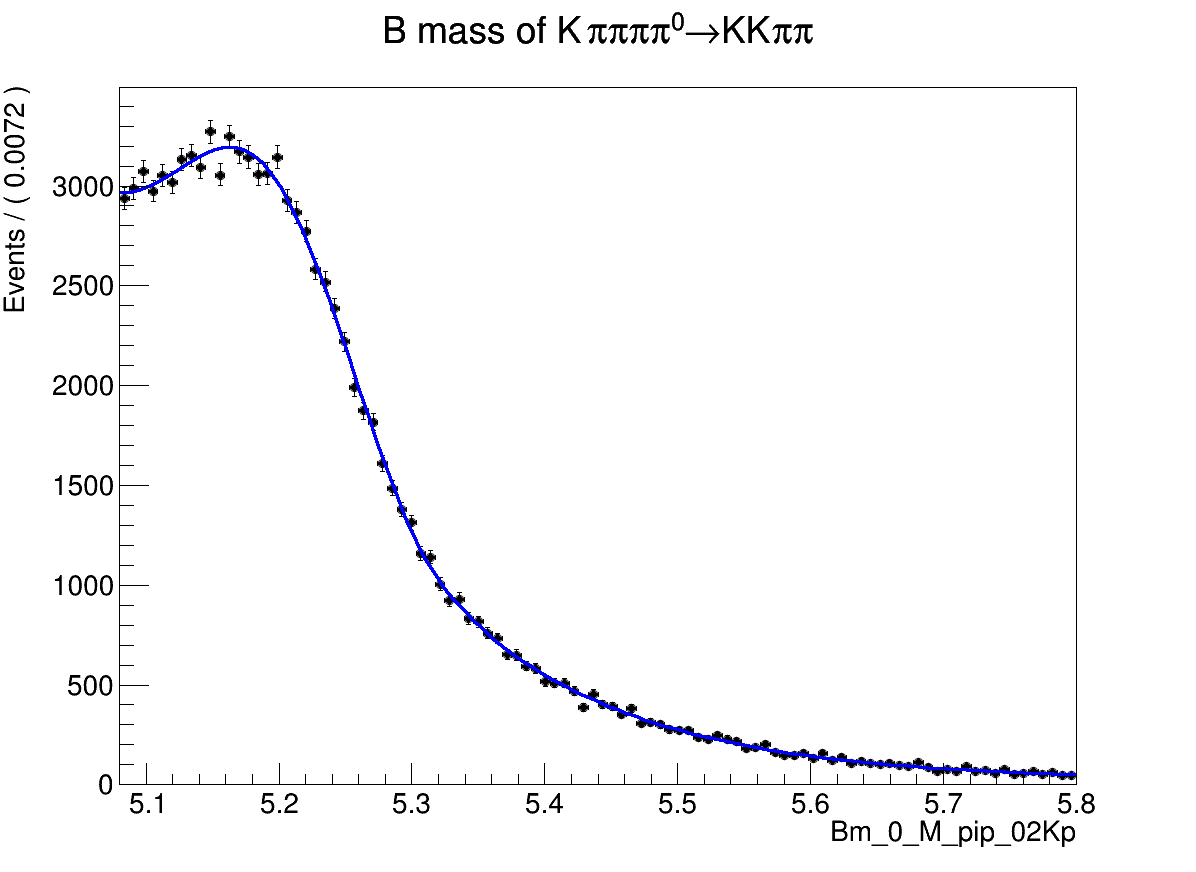
\includegraphics[width = 1.0\textwidth]{Plots/Kpipipipi0BMassB2DpiD2Kpipipi_RapidSim.png}
      \caption{RapidSim}
    \end{subfigure}%
    \begin{subfigure}{0.50\textwidth}
      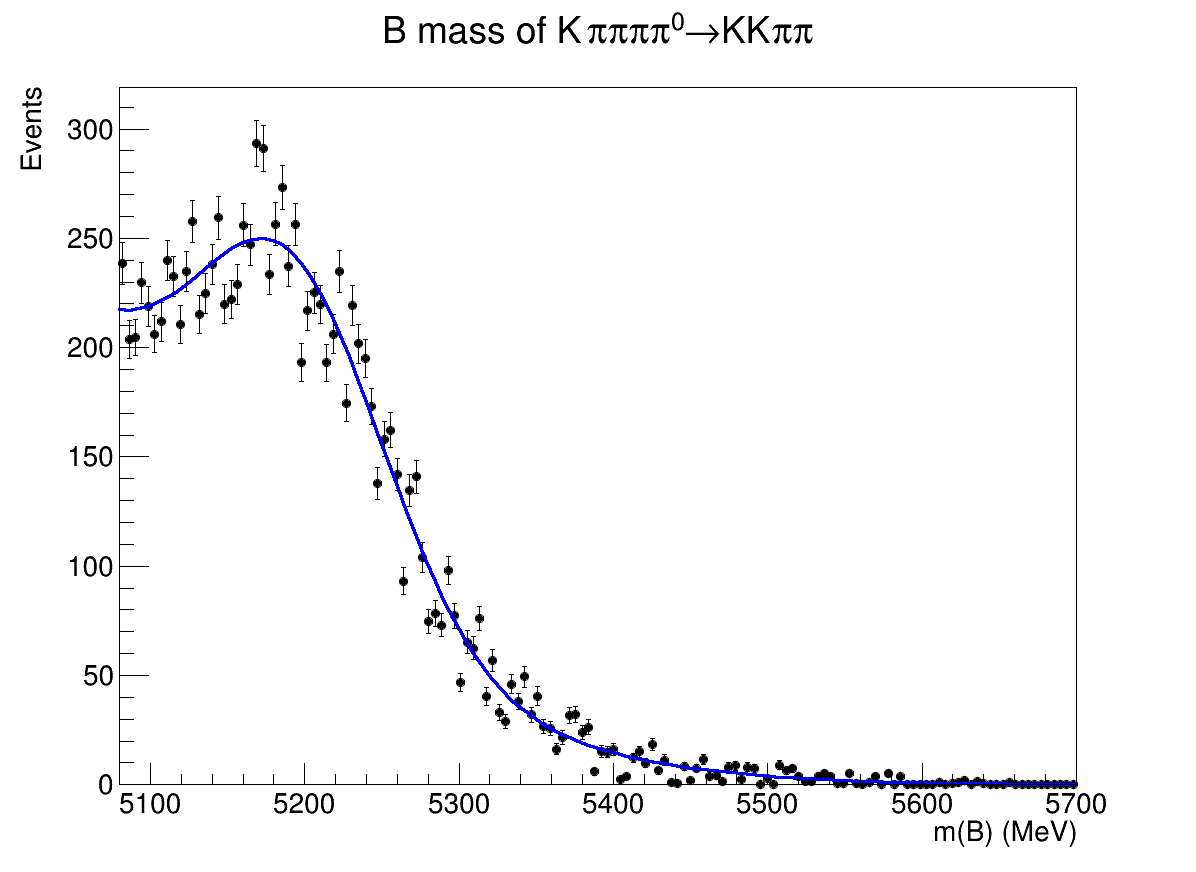
\includegraphics[width = 1.0\textwidth]{Plots/Kpipipipi0BMassB2DpiD2Kpipipi.png}
      \caption{Full LHCb simulation}
    \end{subfigure}
  \end{figure}
\end{frame}

\subsection{Some minor changes and improvements}
\begin{frame}{Some minor changes and improvements}
  \begin{enumerate}
    \setlength\itemsep{1.5em}
    \item{$K_S$ veto for $D\to\pi\pi\pi\pi$ added to match the CLEO-c $F_+$ analysis}
    \item{Fit bias is corrected for}
    \item{Fit range reduced from $\SI{5800}{\mega\eV}$ to $\SI{5700}{\mega\eV}$}
    \item{BPGGSZ and quasi-GLW correlations accounted for}
  \end{enumerate}
\end{frame}

\subsection{Systematic uncertainties}
\begin{frame}{Systematic uncertainties}
  \begin{enumerate}
    \setlength\itemsep{1.0em}
    \item{$c_i$/$s_i$ systematic uncertainty from modelling}
    \begin{itemize}
      \item{Strategy: Generate toys with $c_i$/$s_i$ from older CLEO model, fit with $c_i$/$s_i$ from LHCb model}
      \item{Largest systematic uncertainty}
      \item{Will be replaced when BESIII results become available}
    \end{itemize}
    \item{Charmless background: Vary the total yield and fractional bin yields}
    \item{$K\pi\pi\pi\pi^0$: Vary bin distribution from $D^0$-like to $D^0$+$\bar{D^0}$-like}
    \item{D mixing: Bias from toy fit}
    \begin{itemize}
      \item{More or less negligible when $F_i$ are floated}
      \item{Relatively large if $F_i$ are fixed}
    \end{itemize}
    \item{All quasi-GLW systematic studies finished}
  \end{enumerate}
\end{frame}

\begin{frame}{Summary of all BPGGSZ systematic uncertainties}
  \begin{center}
    Uncertainties of BPGGSZ CP observables in units of $10^{-2}$
  \end{center}
  \scriptsize
  \vspace{0.02cm}
  \begin{center}
    \begin{tabular}{lcccccc} 
      \hline
      Source & $x_-^{DK}$ & $y_-^{DK}$ & $x_+^{DK}$ & $y_+^{DK}$ & $x_\xi^{D\pi}$ & $y_\xi^{D\pi}$ \\
      \hline
      Statistical                                   & 2.99  & 3.50  & 2.58  & 3.10  & 4.07  & 4.89  \\
      \hline
      $c_i$, $s_i$                                  & 0.14  & 3.82  & 1.78  & 1.03  & 0.01  & 0.71  \\
      \hline
      $B^\pm\to D\mu\nu$   background               & 0.07  & 0.06  & 0.08  & 0.30  & 0.17  & 0.00  \\
      $D\to K(X)l\nu_l$ background                  & 0.08  & 0.00  & 0.73  & 0.14  & 0.27  & 0.44  \\
      $D\to K\pi\pi\pi$ background                  & 0.25  & 0.00  & 0.73  & 0.06  & 0.07  & 0.27  \\
      $D\to K\pi\pi\pi\pi^0$ background             & 0.37  & 0.07  & 0.20  & 0.04  & 0.45  & 0.19  \\
      $\Lambda_b$ background                        & 0.10  & 0.06  & 0.06  & 0.26  & 0.15  & 0.07  \\
      Bin dependent mass shape                      & 0.06  & 0.12  & 0.13  & 0.12  & 0.24  & 0.12  \\
      Charmless background                          & 0.15  & 0.18  & 0.14  & 0.16  & 0.01  & 0.01  \\
      Fit bias                                      & 0.00  & 0.00  & 0.00  & 0.00  & 0.00  & 0.00  \\
      Fixed yield fractions                         & 0.02  & 0.03  & 0.02  & 0.02  & 0.01  & 0.01  \\
      Low mass physics effects                      & 0.15  & 0.21  & 0.05  & 0.20  & 0.03  & 0.44  \\
      Mass shape                                    & 0.03  & 0.03  & 0.02  & 0.02  & 0.04  & 0.01  \\
      PID Efficiency                                & 0.03  & 0.03  & 0.02  & 0.02  & 0.04  & 0.01  \\
      $D$ mixing                                    & 0.00  & 0.02  & 0.01  & 0.02  & 0.00  & 0.00  \\
      \hline
      Total LHCb systematic                         & 0.52  & 0.32  & 1.08  & 0.52  & 0.63  & 0.72  \\
      \hline
      Total systematic                              & 0.54  & 3.83  & 2.08  & 1.15  & 0.63  & 1.01  \\
      \hline
    \end{tabular}
  \end{center}
\end{frame}

\begin{frame}{Summary of all quasi-GLW systematic uncertainties}
  \begin{center}
    Uncertainties of quasi-GLW CP observables in units of $10^{-2}$
  \end{center}
  \footnotesize
  \vspace{0.02cm}
  \begin{center}
    \begin{tabular}{lcccccc} 
      \hline
      Source & $A_K^{KK\pi\pi}$ & $A_\pi^{KK\pi\pi}$ & $A_K^{\pi\pi\pi\pi}$ & $A_\pi^{\pi\pi\pi\pi}$ & $R_{\rm CP}^{KK\pi\pi}$ & $R_{\rm CP}^{\pi\pi\pi\pi}$ \\
      \hline
      Statistical                                   & 23.49 & 13.36 &  5.56 &  3.12 & 24.54 & 14.46 \\
      \hline
      Charmless background                          &  1.20 &  0.44 &  0.01 &  0.00 & 13.72 &  8.43 \\
      External parameters                           &  0.98 &  0.99 &  0.74 &  0.74 &  3.98 &  3.96 \\
      Fixed yield fractions                         &  0.11 &  0.08 &  0.02 &  0.00 &  1.32 &  1.44 \\
      Mass shape                                    &  0.27 &  0.20 &  0.03 &  0.02 &  3.11 &  3.05 \\
      PID efficiency                                &  0.18 &  0.12 &  0.01 &  0.00 &  2.55 &  1.64 \\
      \hline
      Total systematic                              &  1.59 &  1.11 &  0.74 &  0.74 & 14.90 & 10.04 \\
      \hline
    \end{tabular}
  \end{center}
\end{frame}

\section{CP fit results, including central values (analysis not blind)}
\begin{frame}{CP fit results}
  \begin{center}
    {\huge CP fit results}
  \end{center}
\end{frame}

\begin{frame}{GLW CP observables}
  \begin{figure}
    \centering
    \begin{subfigure}{0.4\textwidth}
      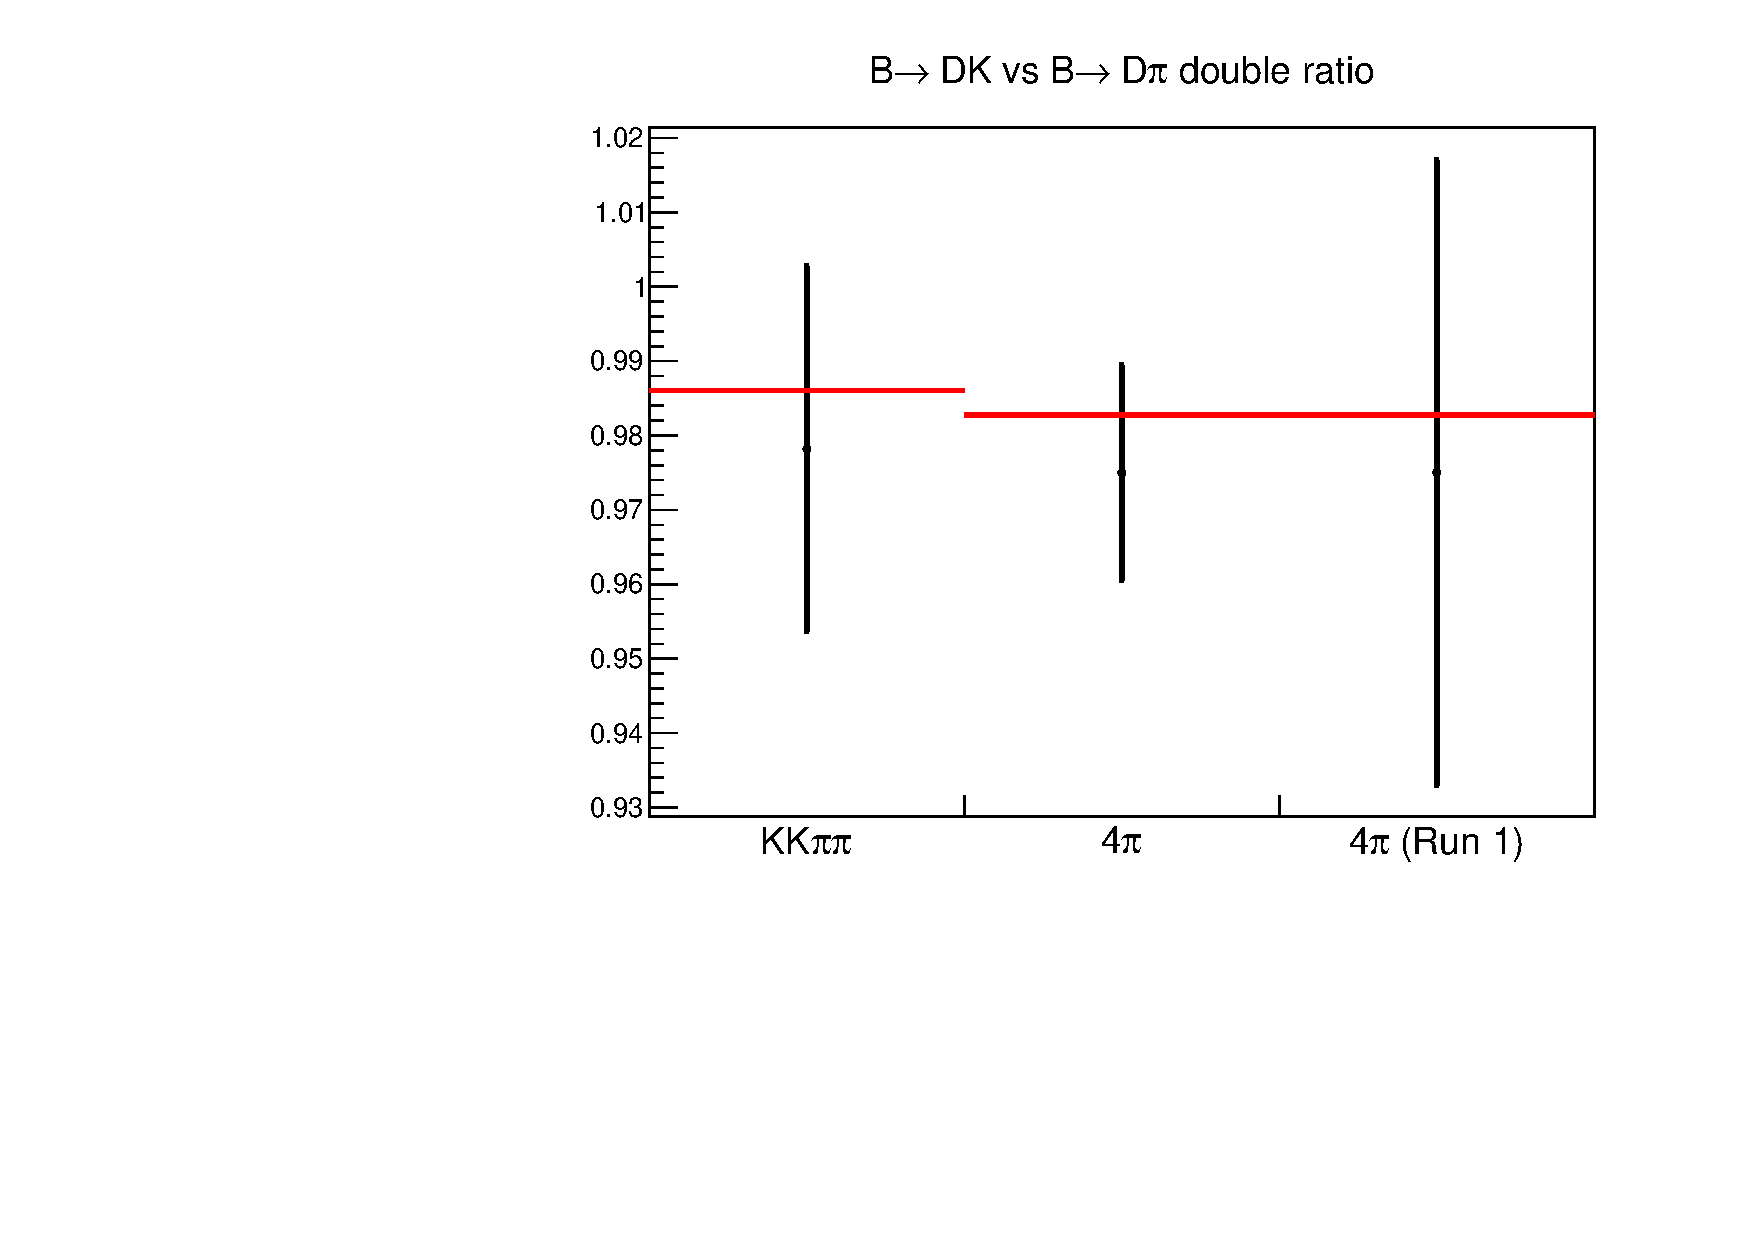
\includegraphics[width = 1.0\textwidth]{Plots/R_CP.pdf}
    \end{subfigure}
    \begin{subfigure}{0.4\textwidth}
      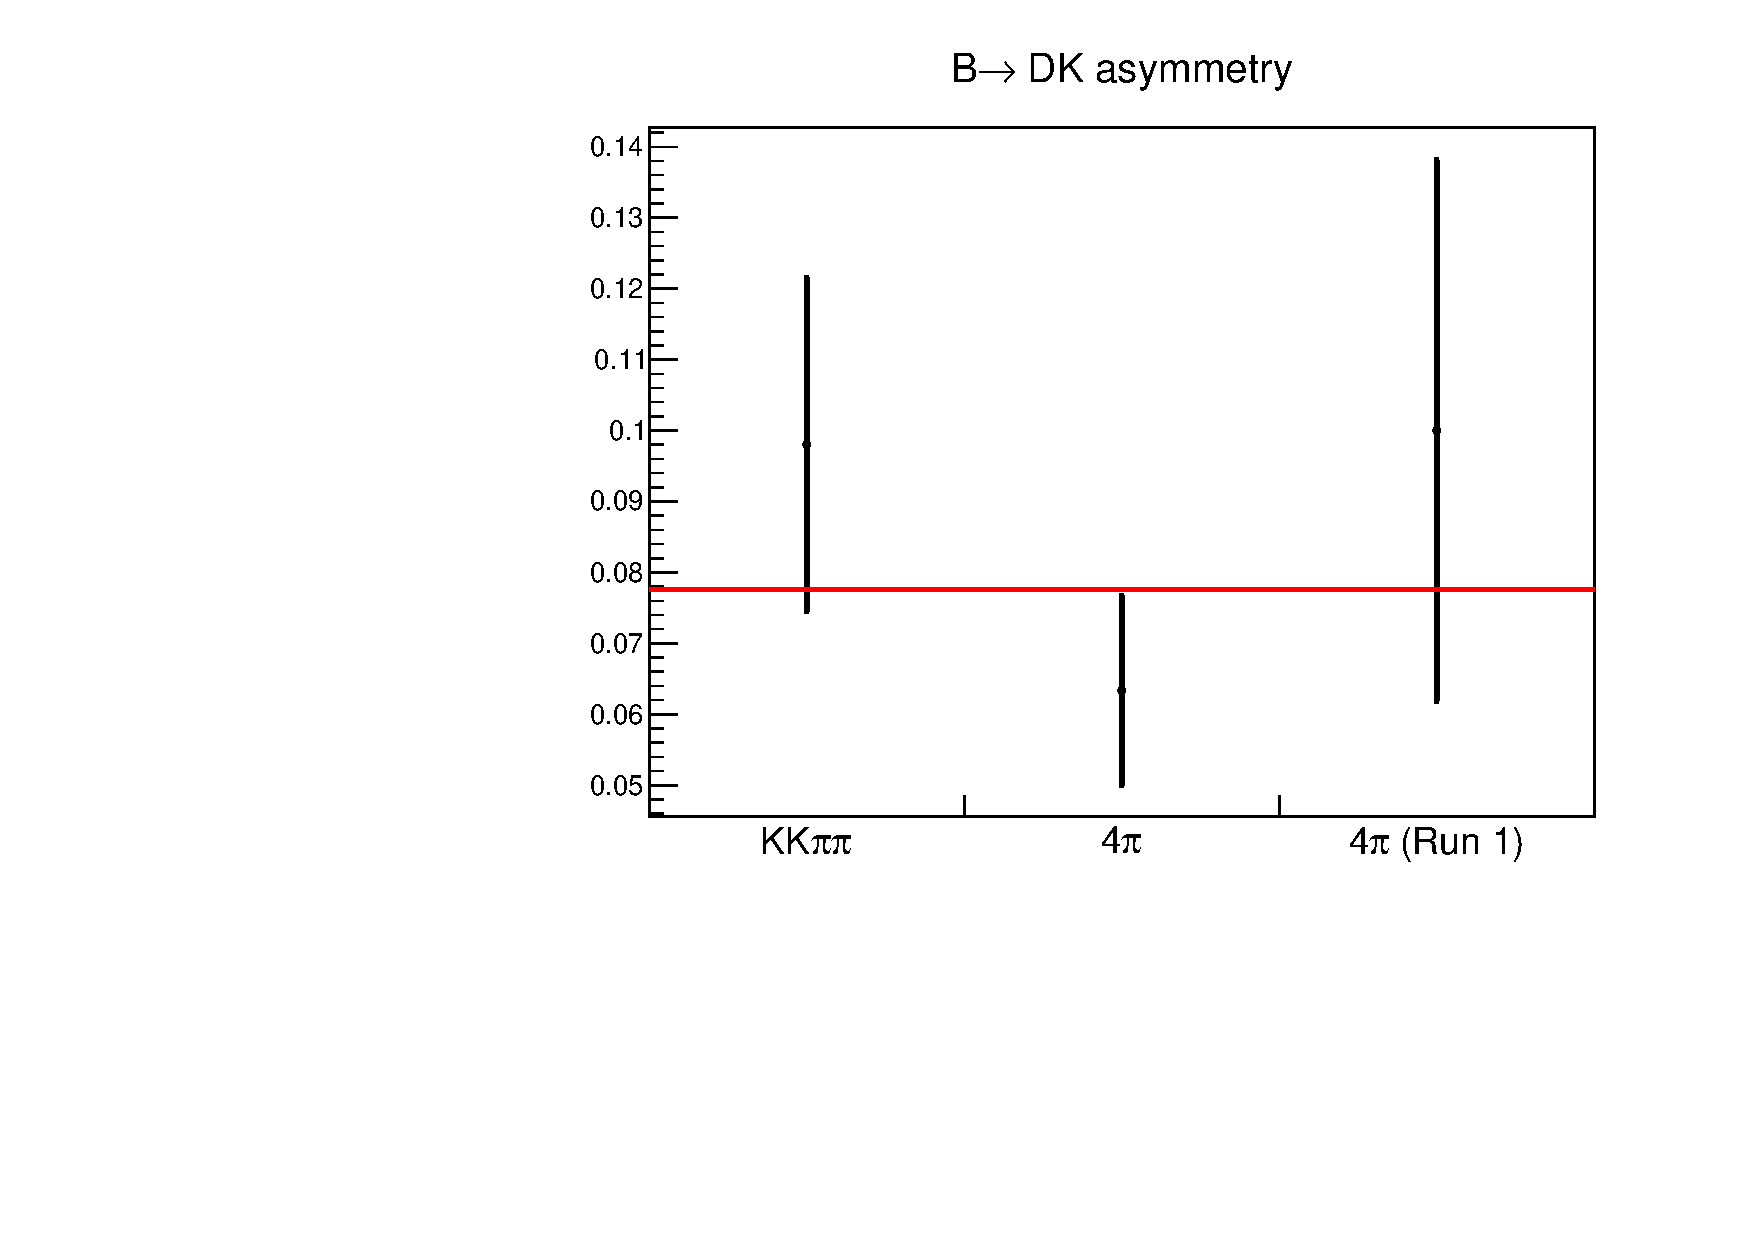
\includegraphics[width = 1.0\textwidth]{Plots/B2DK_Asymmetry.pdf}
    \end{subfigure}%
    \begin{subfigure}{0.4\textwidth}
      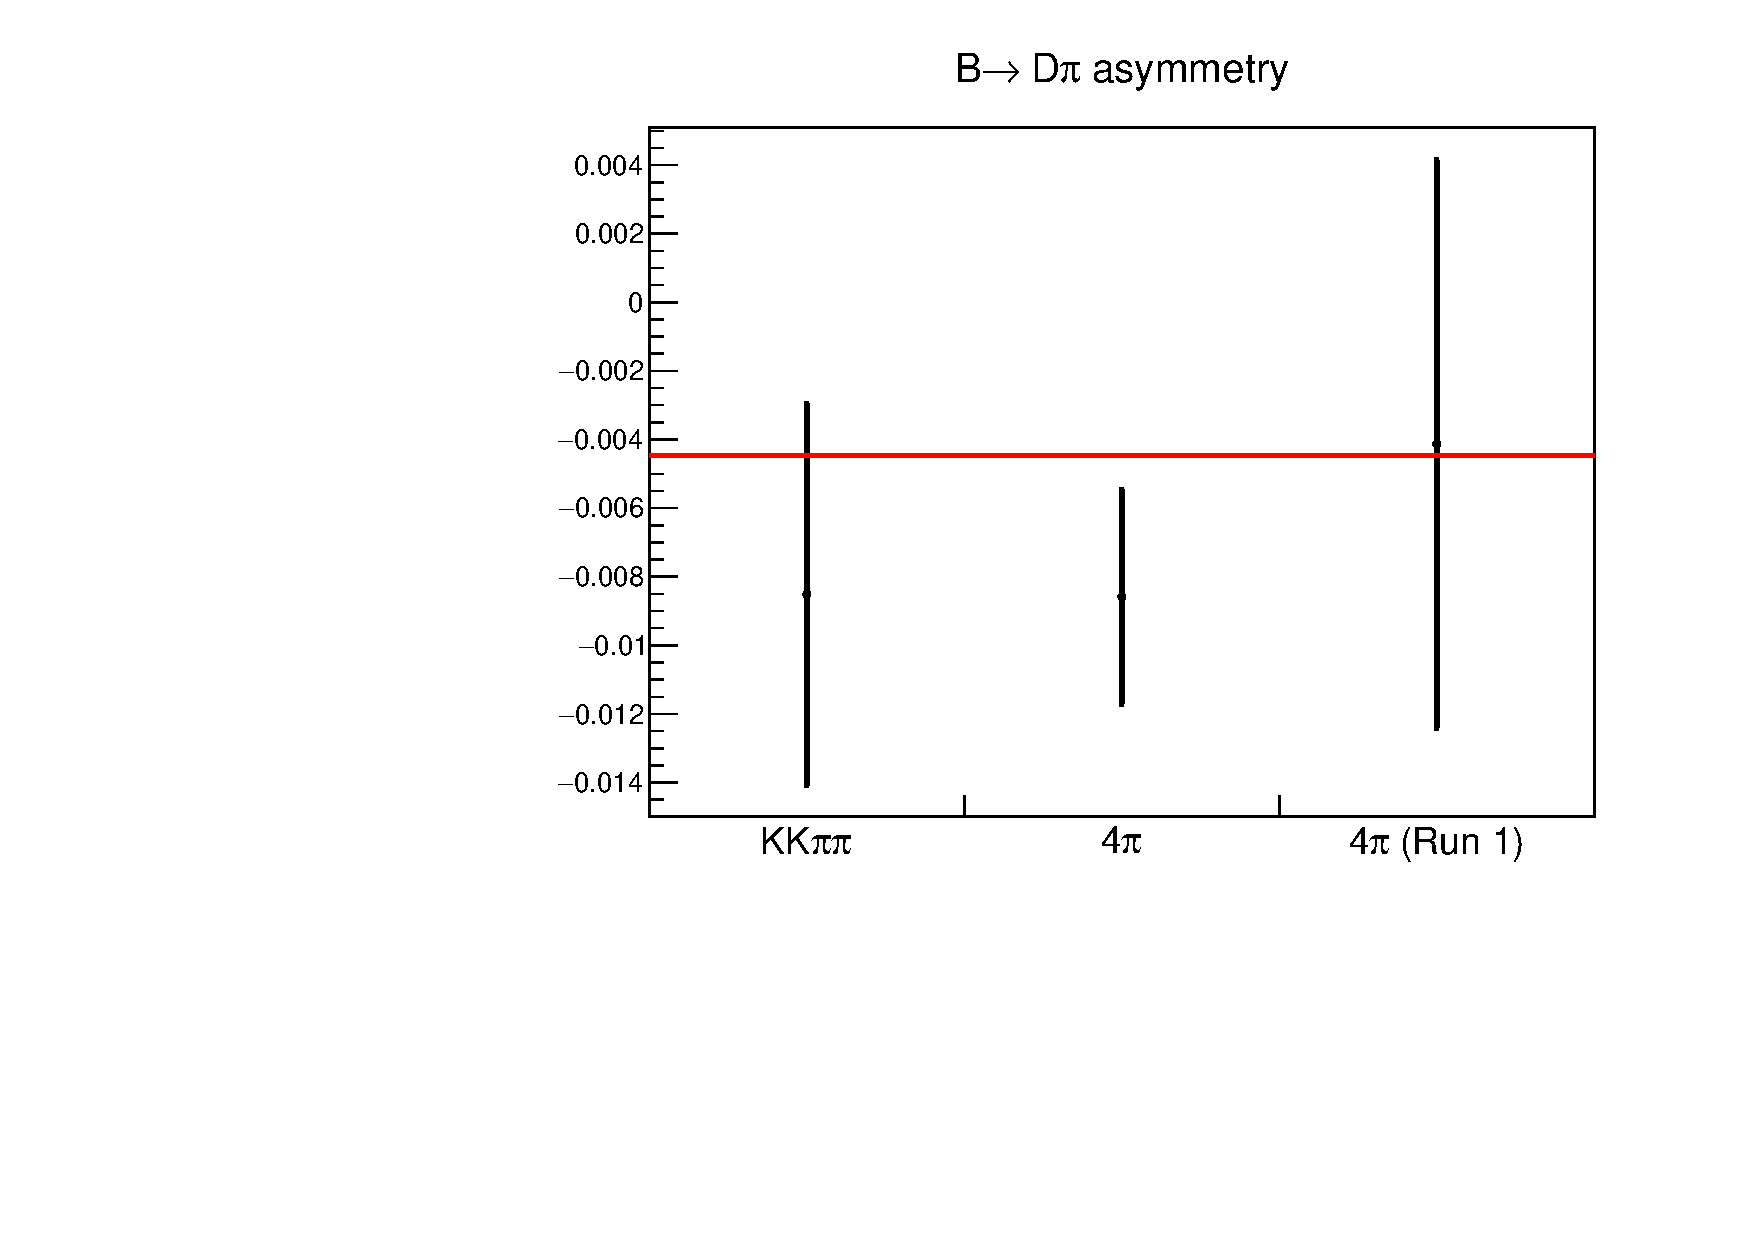
\includegraphics[width = 1.0\textwidth]{Plots/B2Dpi_Asymmetry.pdf}
    \end{subfigure}
  \end{figure}
  \begin{center}
    Red line: Prediction for CP observables using $\gamma$+charm combination
  \end{center}
\end{frame}

\begin{frame}{Binned CP fit}
  \begin{itemize}
    \setlength\itemsep{0.0em}
    \item{PDF shape parameters fixed from global fit}
    \item{$2$ charges, 2 $B$ decays, $2\times 8$ bins $\implies$ $64$ categories}
    \item{Nuisance parameters:}
    \begin{itemize}
      \item{Combinatorial and low mass background ($2\times 64$ parameters)}
      \item{$F_i$ ($15$ parameters)}
      \item{Yield normalization for each charge and $B$ decay ($4$ parameters)}
    \end{itemize}
    \item{$6$ CP observables $\implies$ 153 free parameters in total}
  \end{itemize}
  \begin{figure}
    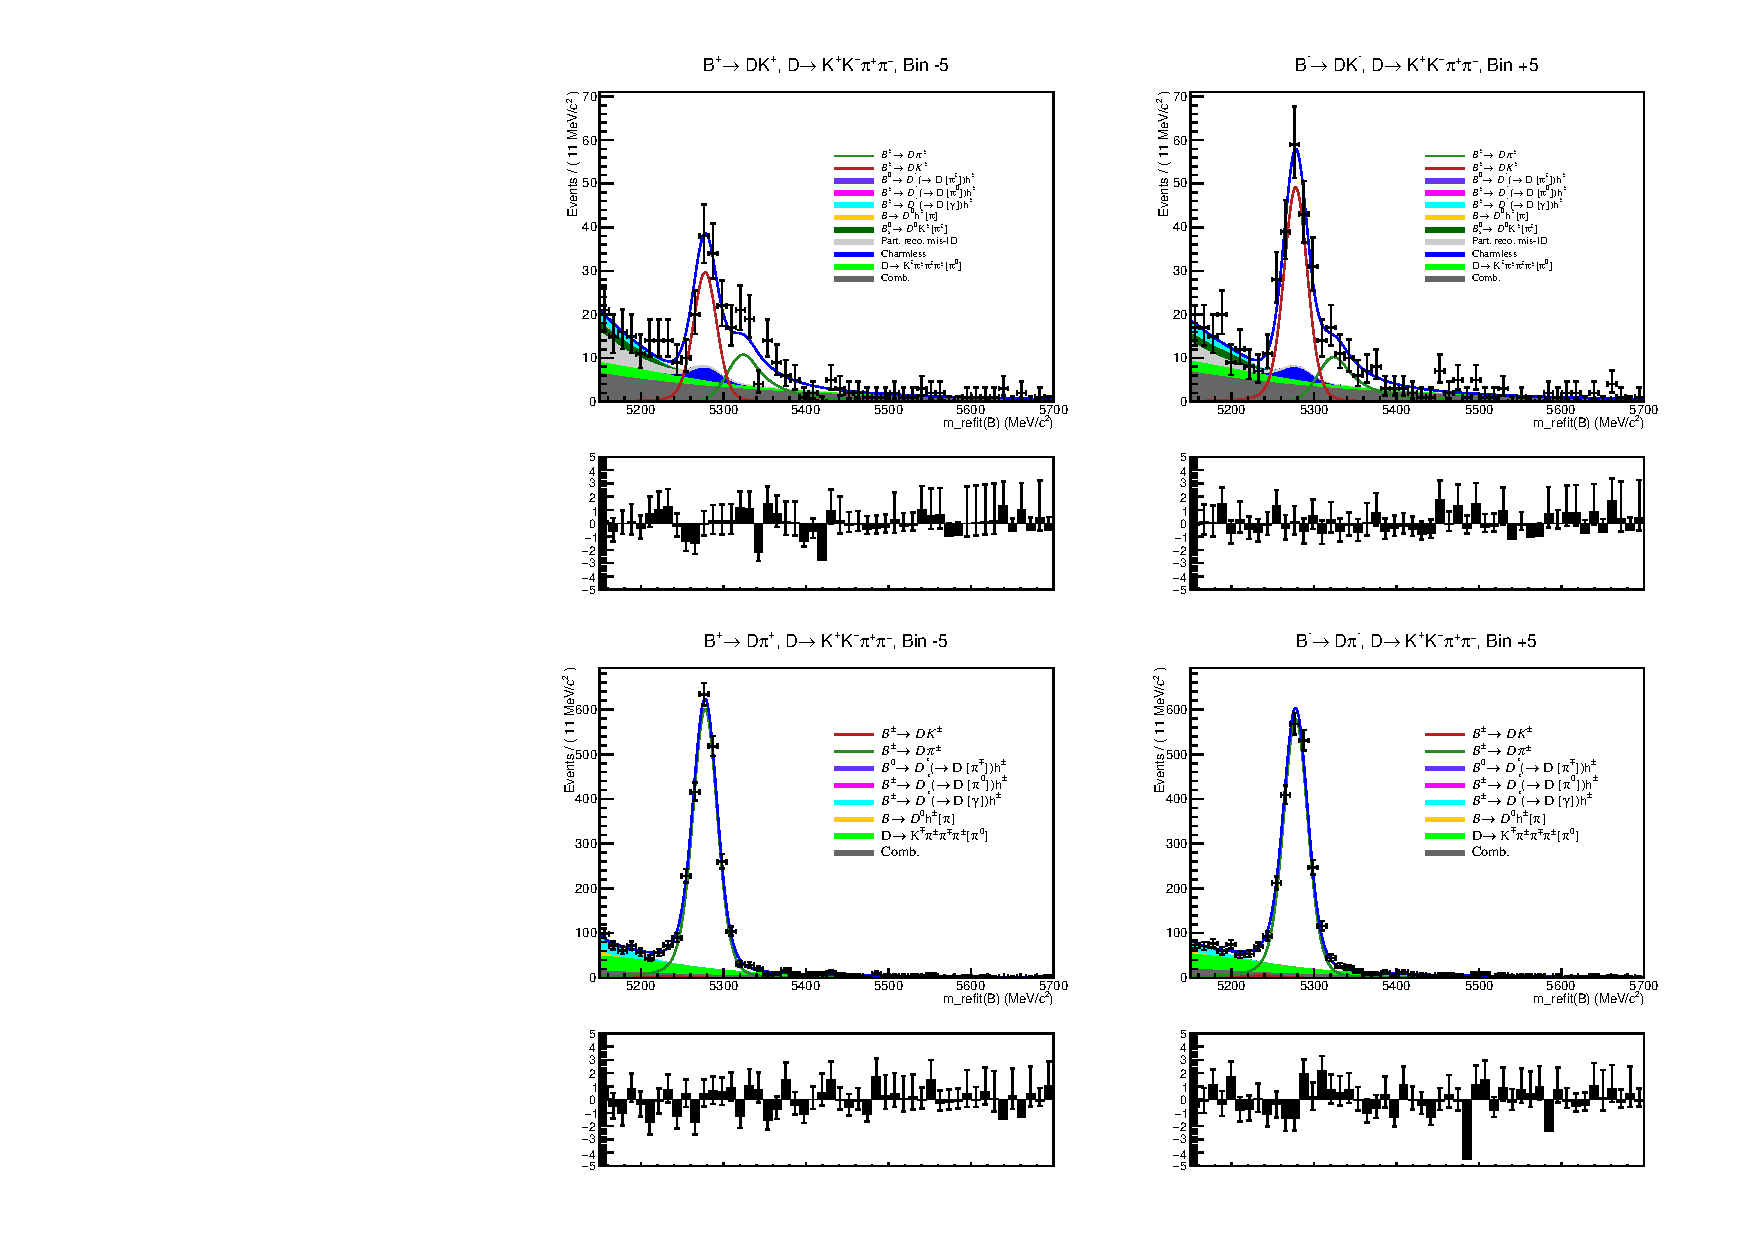
\includegraphics[width = 1.0\textwidth, clip = true, trim = {0 13cm 0 0}]{Plots/d2kkpipi_fiveL_binm5.pdf}
  \end{figure}
\end{frame}

\begin{frame}{CP observables result}
  \begin{figure}
    \centering
    \begin{subfigure}{0.50\textwidth}
      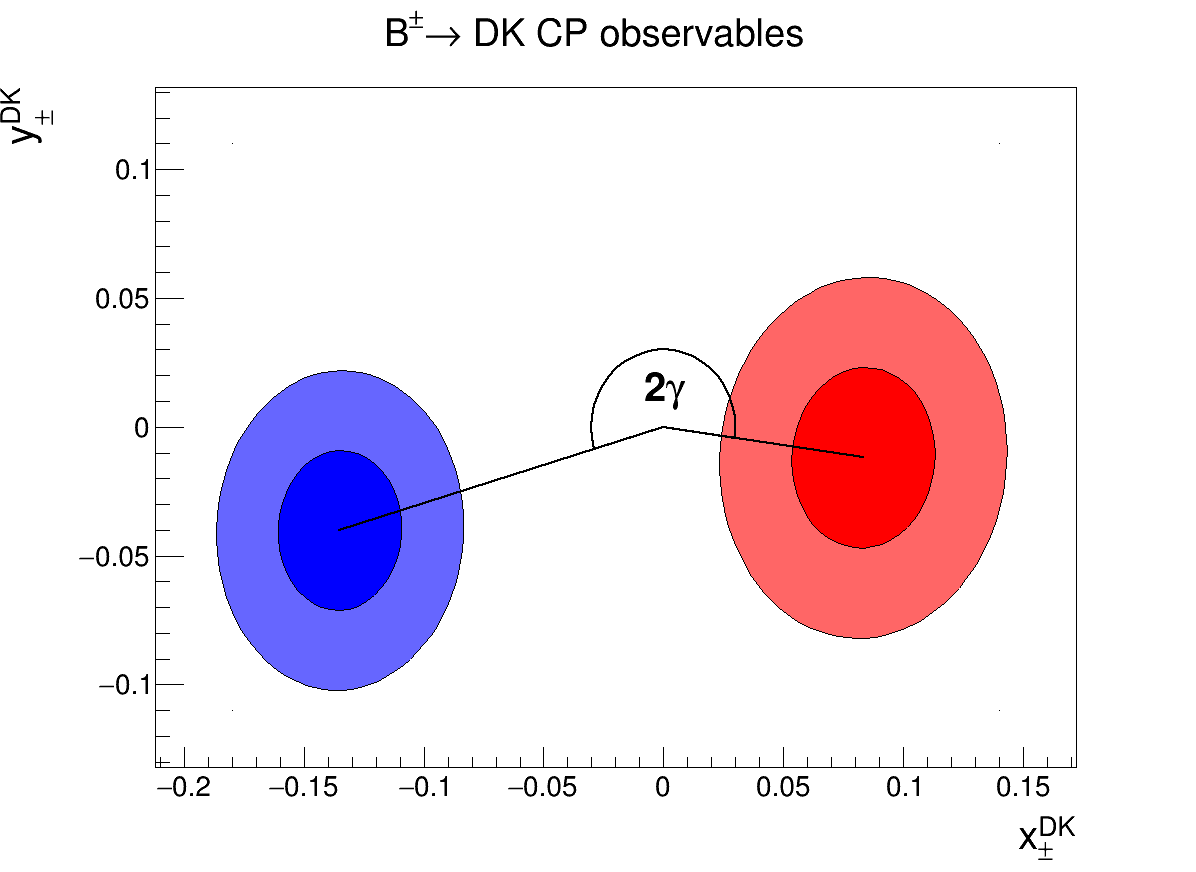
\includegraphics[width = 1.0\textwidth]{Plots/B2DK_CP_Observables_Contours.png}
    \end{subfigure}%
    \begin{subfigure}{0.50\textwidth}
      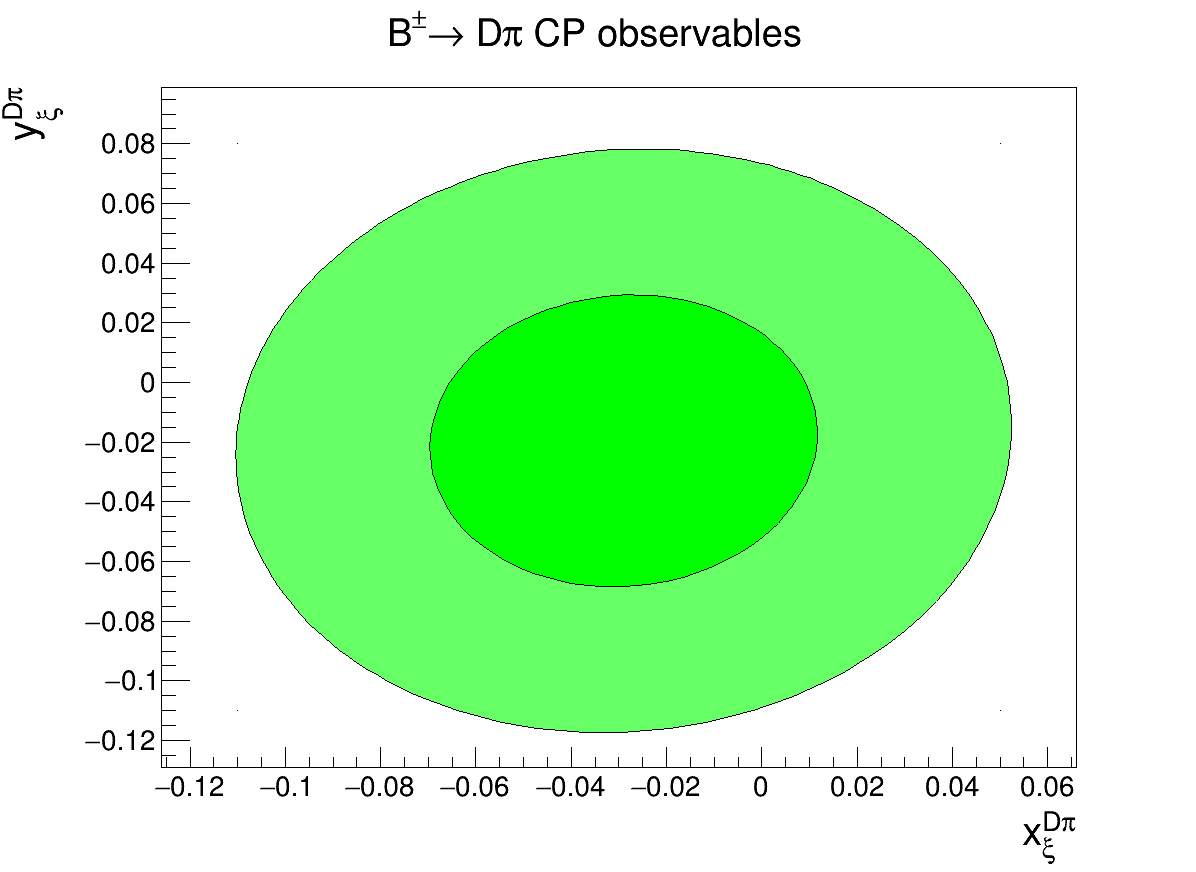
\includegraphics[width = 1.0\textwidth]{Plots/B2Dpi_CP_Observables_Contours.png}
    \end{subfigure}
  \end{figure}
  \begin{center}
    \huge \vphantom{Could there be a sign error in $s_i$?}
  \end{center}
\end{frame}

\begin{frame}{CP observables result}
  \begin{figure}
    \centering
    \begin{subfigure}{0.50\textwidth}
      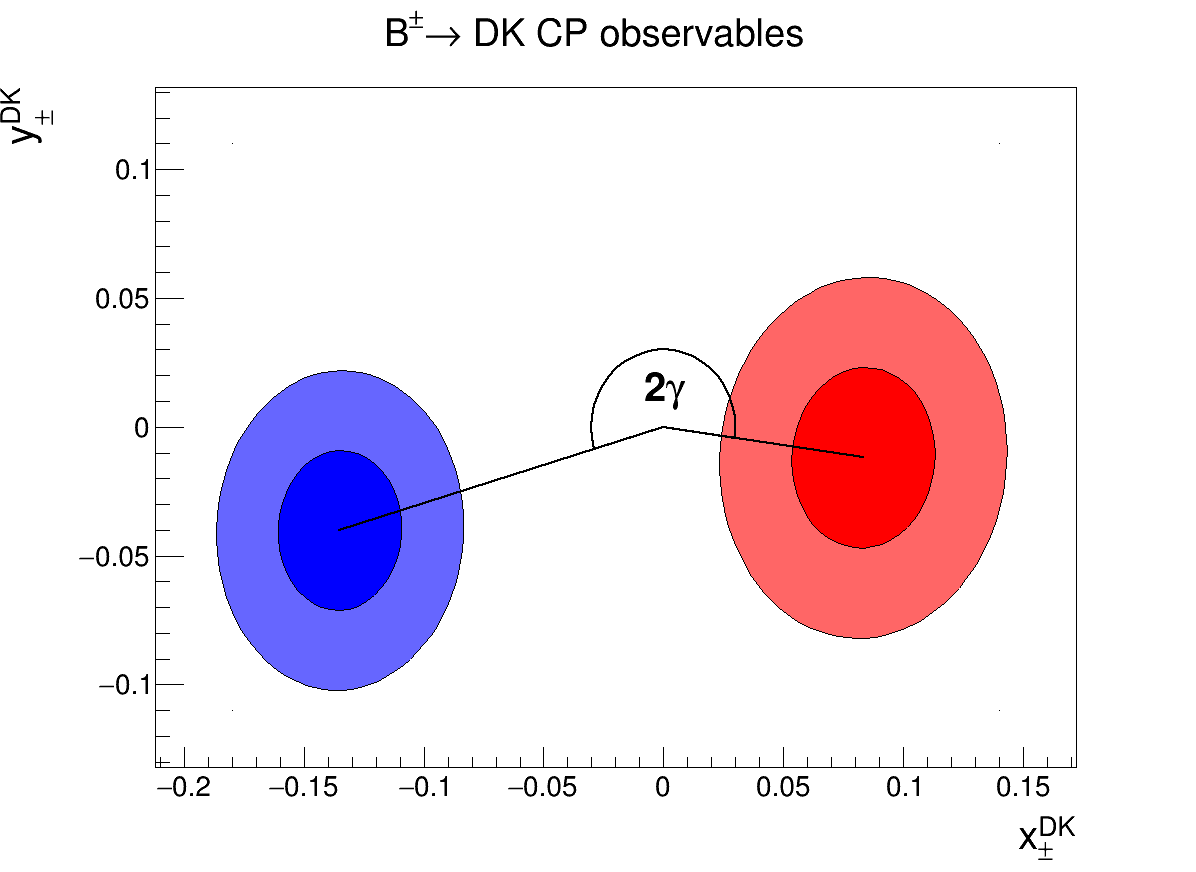
\includegraphics[width = 1.0\textwidth]{Plots/B2DK_CP_Observables_Contours.png}
    \end{subfigure}%
    \begin{subfigure}{0.50\textwidth}
      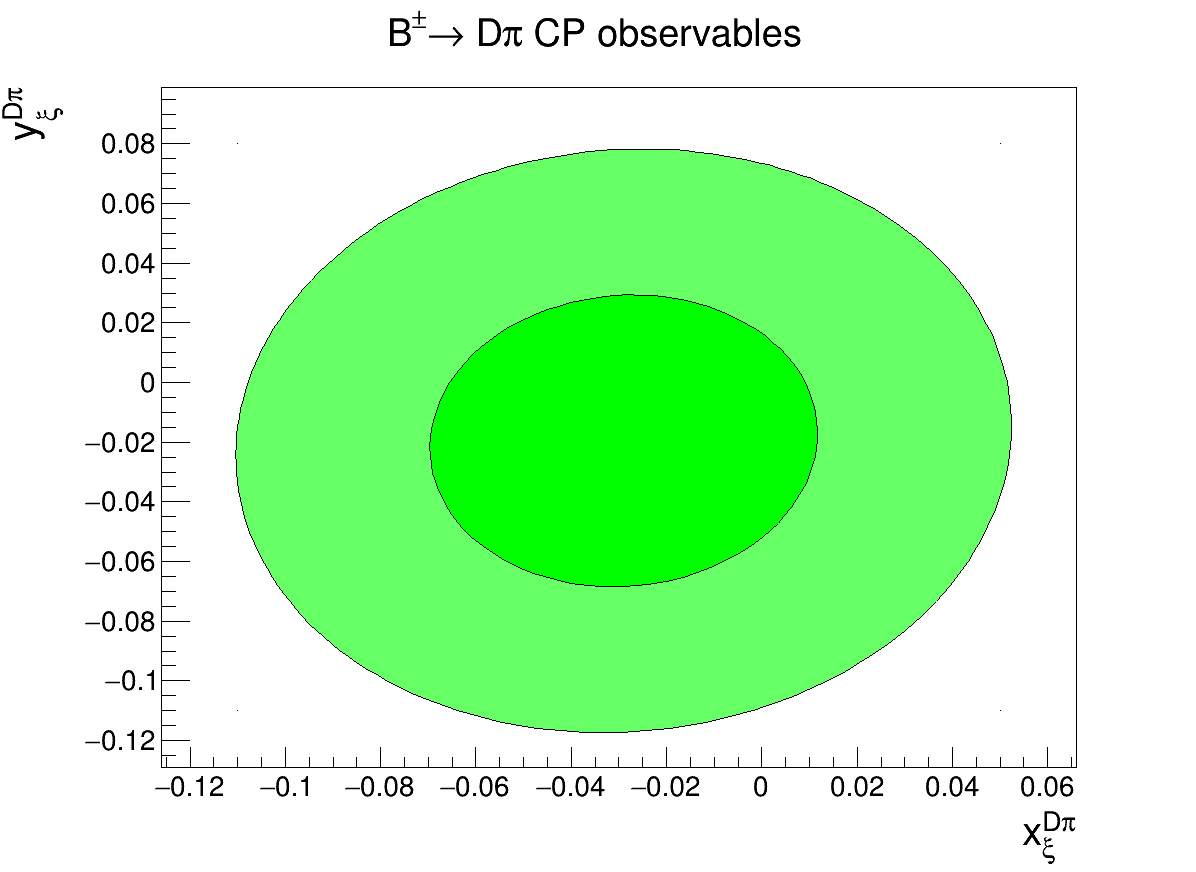
\includegraphics[width = 1.0\textwidth]{Plots/B2Dpi_CP_Observables_Contours.png}
    \end{subfigure}
  \end{figure}
  \begin{center}
    \huge Could there be a sign error in $s_i$?
  \end{center}
\end{frame}

\begin{frame}{Interpretation}
  \begin{figure}
    \centering
    \begin{subfigure}{0.50\textwidth}
      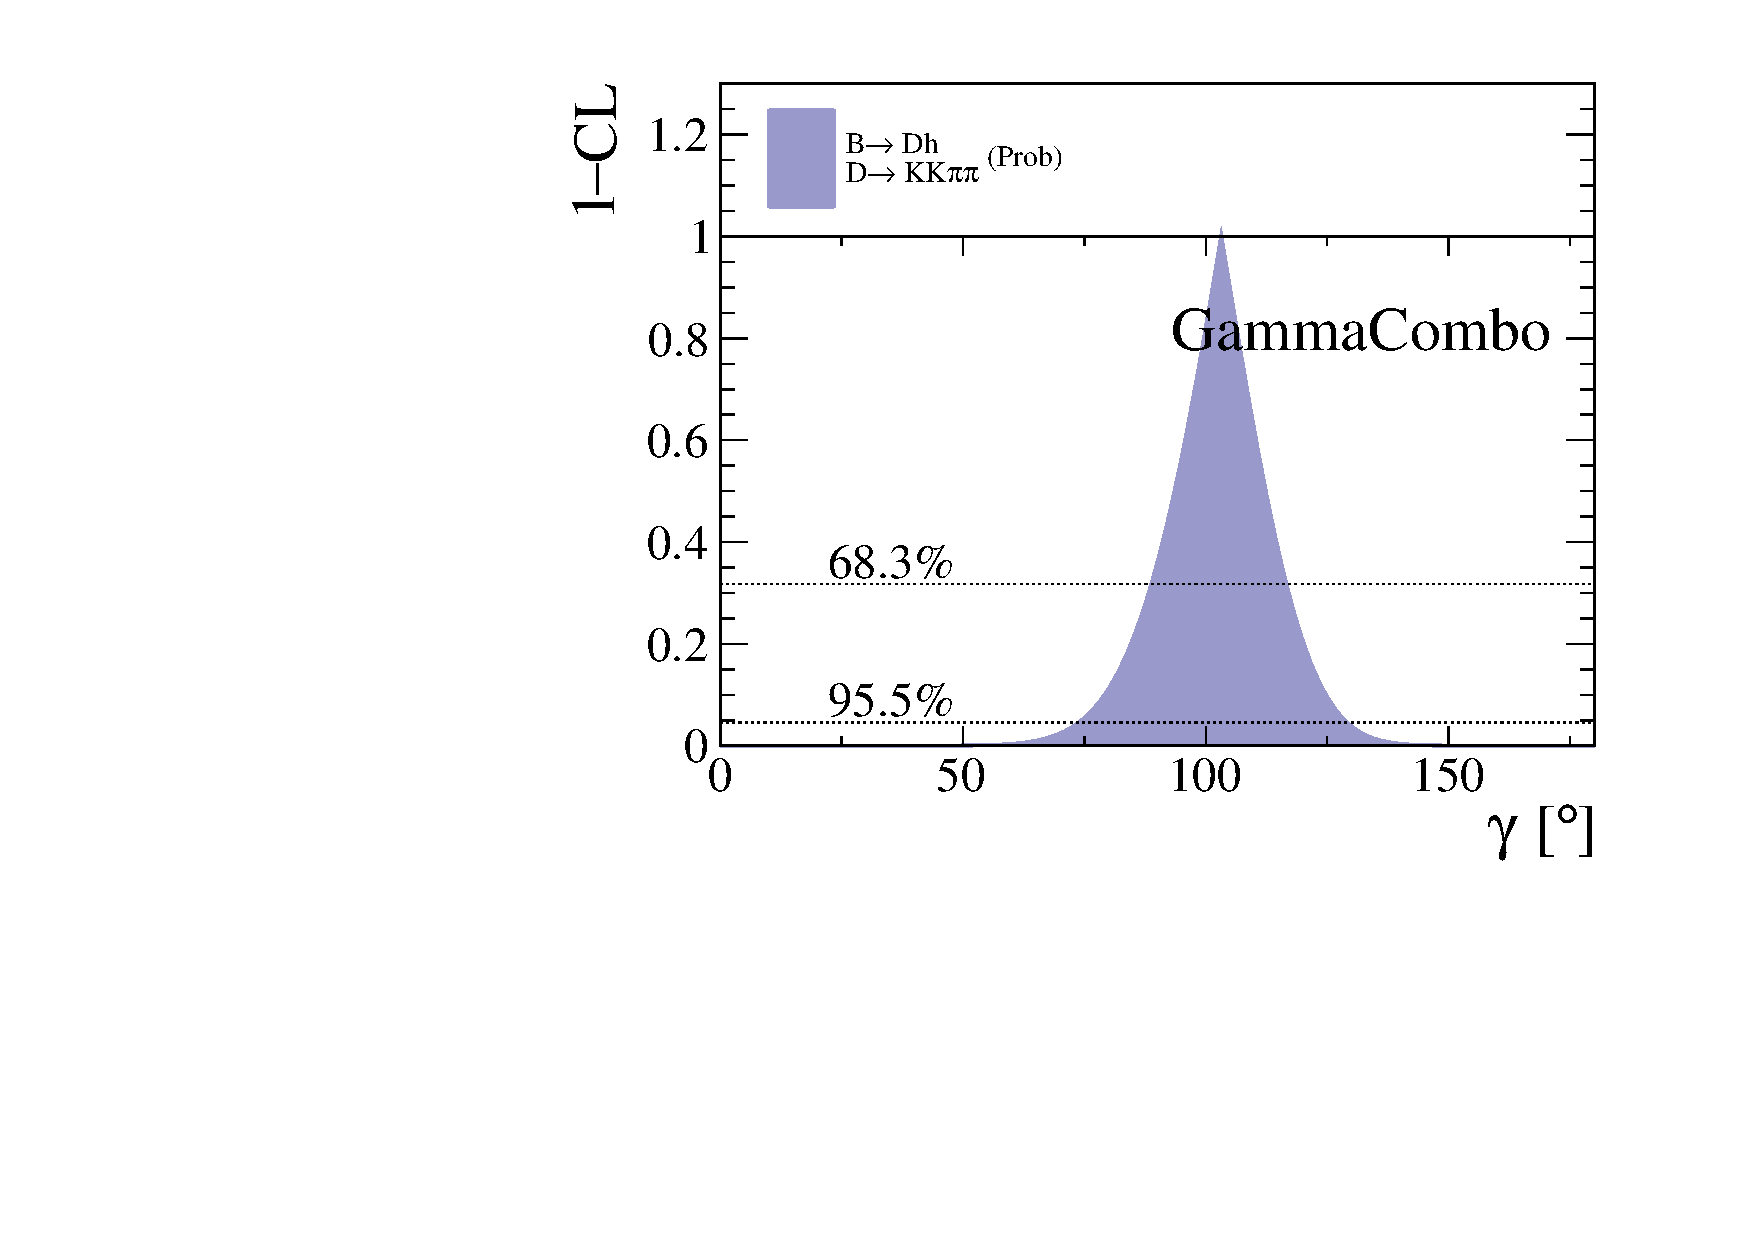
\includegraphics[width = 1.0\textwidth]{Plots/cartesian_KKpipi_GGSZ_gamma.pdf}
    \end{subfigure}%
    \begin{subfigure}{0.50\textwidth}
      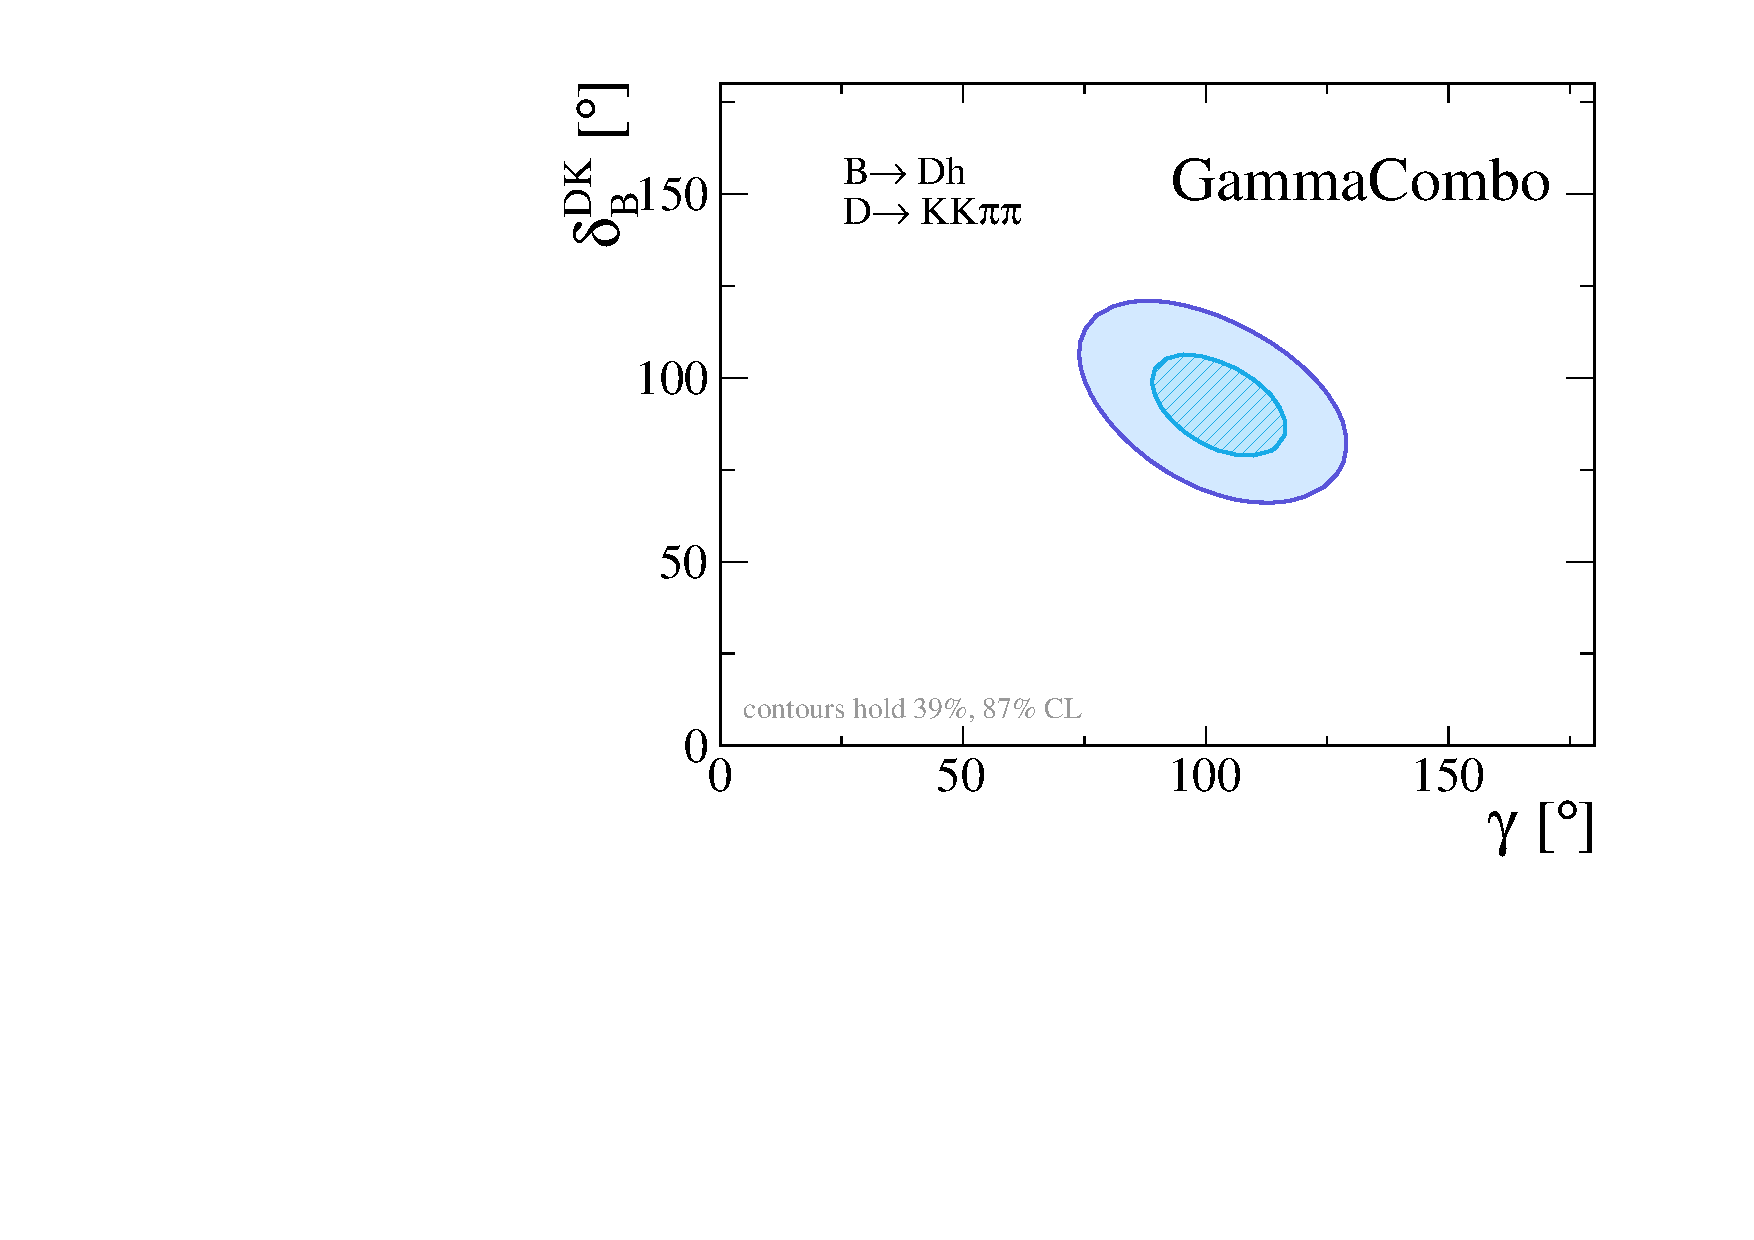
\includegraphics[width = 1.0\textwidth]{Plots/cartesian_KKpipi_GGSZ_gamma_d_dk.pdf}
    \end{subfigure}
  \end{figure}
  \vspace{-0.75cm}
  \begin{align*}
    \gamma =& (103\pm14)^\circ \\
    \delta_B^{DK} =& (92\pm14)^\circ \\
    r_B^{DK} =& 0.117\pm0.020 \\
    \delta_B^{D\pi} =& (296\pm84)^\circ \\
    r_B^{D\pi} =& 0.004\pm0.005
  \end{align*}
\end{frame}

\section{Summary of $KK\pi\pi$ analysis}
\begin{frame}{Summary of $KK\pi\pi$ analysis}
  \begin{center}
    {\huge Summary of $KK\pi\pi$ analysis}
  \end{center}
\end{frame}

\begin{frame}{Summary of $KK\pi\pi$ analysis}
  \begin{itemize}
    \item{Measured CP observables:}
  \end{itemize}
  \vspace{-0.2cm}
  \begin{align*}
    x_-^{DK} =& (8.3 \pm 3.0 \pm 0.5 \pm 0.1)\times 10^{-2}, \\
    y_-^{DK} =& (-1.2 \pm 3.5 \pm 0.3 \pm 3.8)\times 10^{-2}, \\
    x_+^{DK} =& (-13.5 \pm 2.6 \pm 1.1 \pm 1.8)\times 10^{-2}, \\
    y_+^{DK} =& (-4.0 \pm 3.1 \pm 0.5 \pm 1.0)\times 10^{-2}, \\
    x_\xi^{D\pi} =& (-2.9 \pm 4.1 \pm 0.6 \pm 0.0)\times 10^{-2}, \\
    y_\xi^{D\pi} =& (-2.0 \pm 4.9 \pm 0.7 \pm 0.7)\times 10^{-2},
  \end{align*}
  \vspace{-0.5cm}
  \begin{itemize}
    \item{Measured physics parameters:}
  \end{itemize}
  \vspace{-0.2cm}
  \begin{align*}
    \gamma =& (103\pm14)^\circ \\
    \delta_B^{DK} =& (92\pm14)^\circ \\
    r_B^{DK} =& 0.117\pm0.020 \\
    \delta_B^{D\pi} =& (296\pm84)^\circ \\
    r_B^{D\pi} =& 0.004\pm0.005
  \end{align*}
\end{frame}

\section{Conclusion and next steps}
\begin{frame}{Conclusion and next steps}
  \begin{center}
    {\huge Conclusion and next steps}
  \end{center}
\end{frame}

\begin{frame}{Conclusion and next steps}
  \begin{itemize}
    \setlength\itemsep{2em}
    \item{Binned $\gamma$ analysis of $B^\pm\to(K^+K^-\pi^+\pi^-)_Dh^\pm$ is ready for RC}
    \item{Quasi-GLW observables of $h^+h^-\pi^+\pi^-$ further constrains $\gamma$}
    \item{All systematics have been evaluated}
    \item{Next steps:}
    \begin{enumerate}
      \item{Understand double peak error distribution in global fit toys}
      \item{Make sure $s_i$ has the correct sign}
    \end{enumerate}
  \end{itemize}
\end{frame}

\begin{frame}{Thank you!}
  \begin{center}
    {\huge Thank you!}
  \end{center}
\end{frame}

\begin{frame}{Backup}
  \begin{center}
    {\huge Backup}
  \end{center}
\end{frame}

\begin{frame}{Double-peaked error distributions}
  \begin{figure}
    \centering
    \vspace{-0.2cm}
    \begin{subfigure}{0.5\textwidth}
      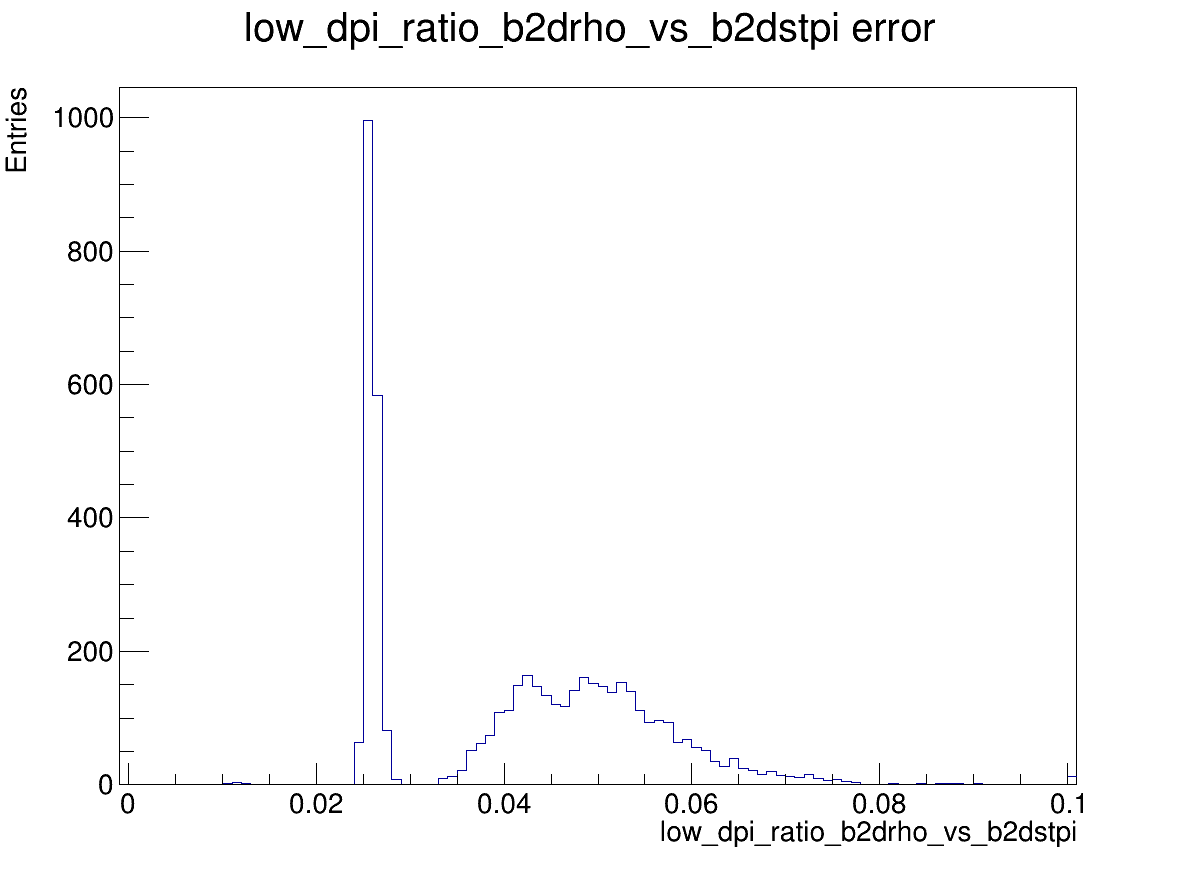
\includegraphics[width = 1.0\textwidth]{Plots/low_dpi_ratio_b2drho_vs_b2dstpi_error.png}
      \caption{$f_{D\pi\pi}^{D\pi}$}
    \end{subfigure}%
    \begin{subfigure}{0.5\textwidth}
      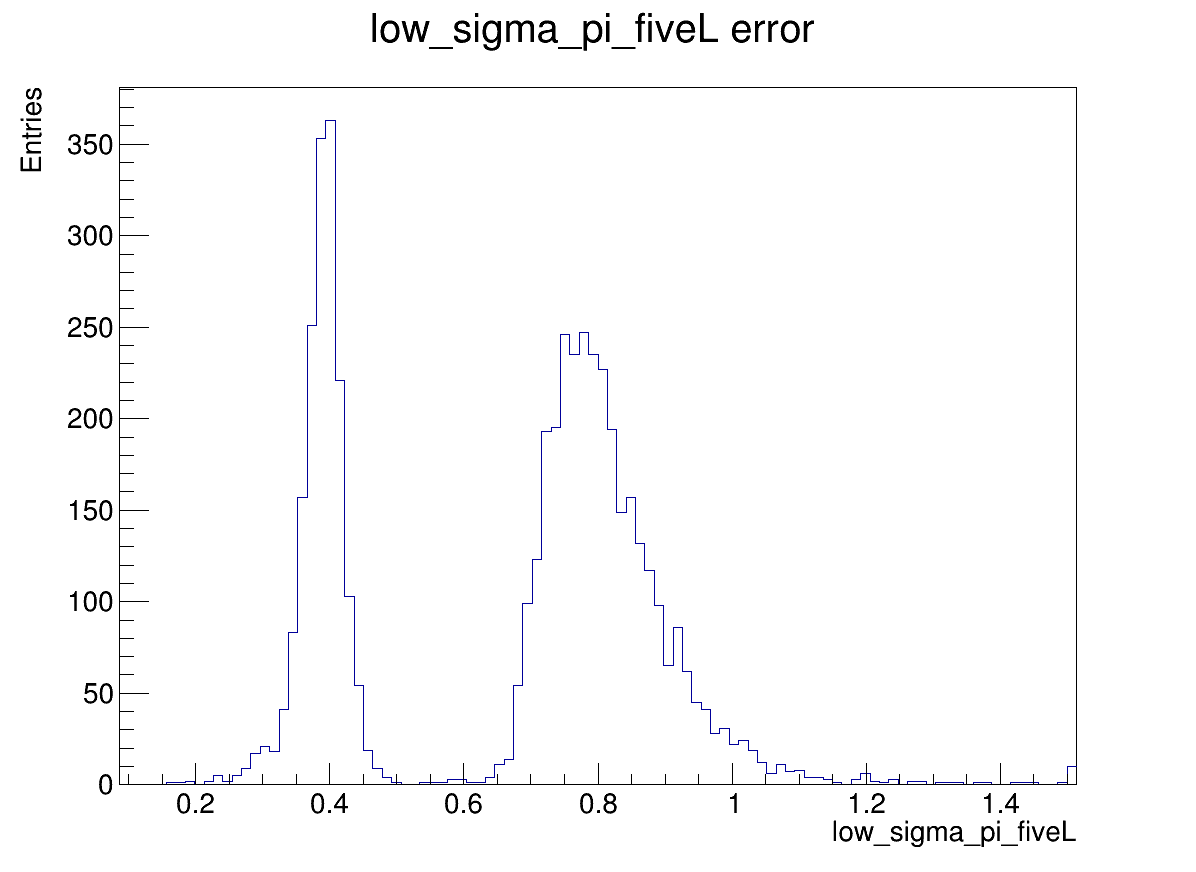
\includegraphics[width = 1.0\textwidth]{Plots/low_sigma_pi_fiveL_error.png}
      \caption{$\sigma_\pi^{\rm low}$}
    \end{subfigure}
  \end{figure}
\end{frame}

\begin{frame}{$s_i$ sign problem}
  \begin{itemize}
    \setlength\itemsep{0.5em}
    \item{Amplitude model gives us: $A(\Phi) = \sum_ka_kS_k(\Phi)$}
    \item{Flavour-tagged LHCb data measures: $\abs{A(\Phi)}^2$}
    \item{$a_k$ phase is fixed from phase convention of $S_k(\Phi)$ lineshapes}
    \item{Physical observable: Interference fractions}
    \begin{itemize}
      \item{Toy fit shows that LHCb and CLEO models are \underline{consistent}}
      \item{Thanks to Tim Evans for checking!}
    \end{itemize}
  \end{itemize}
  \vspace{0.4cm}
  \begin{tabular}{l|c|c}
    Resonance                           & LHCb model phase ($\si{\radian}$) & CLEO model ($\si{\radian}$) \\
    \hline
    $D^0\to[\phi(1020)\rho^0]_{L = 0}$  & $0$ (fixed)                       & $0$ (fixed) \\
    $D^0\to K_1(1400)^+K^-$             & $1.05$                            & $-1.79$ \\
    $D^0\to K_1(1270)^+K^-$             & $2.02$                            & $-2.56$ \\
    \hline
  \end{tabular}
  \vspace{0.4cm}
\end{frame}

\begin{frame}{$s_i$ sign problem}
  \begin{itemize}
    \setlength\itemsep{1.5em}
    \item{BESIII data can determine sign uniquely!}
    \item{Reconstruct $KK\pi\pi$ vs $K_{S,L}\pi\pi$ double tags:}
  \end{itemize}
  \begin{center}
    $M_{i, j}\propto\big(K_iK^\prime_{-j} + K_{-i}K^\prime_j \mp 2\sqrt{K_iK_{-i}K^\prime_jK^\prime_{-j}}(c_ic^\prime_j + s_is^\prime_j)\big)$
  \end{center}
\end{frame}

\begin{frame}{$s_i$ sign problem}
  Cross checks:
  \vspace{0.3cm}
  \begin{enumerate}
    \setlength\itemsep{1.5em}
    \item{Can use BESIII data with $KK\pi\pi$ vs $K_{S, L}\pi\pi$ tags to check $s_i$ sign}
    \item{Same fit code was used in $B\to Dh$, $D\to K_S\pi\pi$ analysis}
    \item{Same code used to bin events in data and in calculation of $c_i$/$s_i$}
    \item{Independent binned fit toys are consistent with AmpGen unbinned fit}
  \end{enumerate}
\end{frame}

\end{document}
